% !TEX TS-program = LuaLaTeX
\documentclass[10pt, oneside, a4paper]{article}

\usepackage[T1]{fontenc}
\usepackage{lmodern}
\usepackage{xcolor}
    \definecolor{gray} {HTML}{363636}
    \definecolor{red}  {HTML}{950009}
    \definecolor{green}{HTML}{0E610A}
    \definecolor{blue} {HTML}{020069}
\usepackage{fontspec}
    \setsansfont{Arial}
\usepackage{amsmath}
\usepackage{titlesec}
    \titleformat*{\section}      {\color{gray}\large\bfseries\sffamily}
    \titleformat*{\subsection}   {\color{gray}\large\bfseries\sffamily}
    \titleformat*{\subsubsection}{\color{gray}\large\bfseries\sffamily}
\usepackage{geometry}
    \geometry{scale={0.75,0.85}}
\usepackage{siunitx}
    \sisetup{locale=FR}
    \sisetup{math-micro=\text{µ},text-micro=µ} % fix
\usepackage{graphicx}
\usepackage{caption}
    \captionsetup{labelfont={bf,sf,color=gray}}
\usepackage{pdfpages}
\usepackage{caption}


% Keep lasts
\usepackage[french]{babel}
    \frenchsetup{SmallCapsFigTabCaptions=false}
\usepackage[expansion]{microtype}
\usepackage[luatex, backref]{hyperref}
    \hypersetup{unicode, colorlinks, breaklinks, urlcolor=red,
                bookmarksopen, bookmarksnumbered}

\renewcommand{\UrlFont}{\small}
\renewcommand{\arraystretch}{1.1}
\setlength{\parskip}{2mm}

\begin{document}

\begin{titlepage}
    \centering
    
\includegraphics[width=0.5\textwidth]{image/logo-ecam.png}\par
    \vspace{1cm}
    
    \rule{\linewidth}{1.5pt}%
    \vspace{5mm}
    {\rm\sffamily\LARGE Rapport de bureau d'étude\par}
    \vspace{3mm}
    {\sffamily\bfseries\LARGE Réalisation d'un amplificateur de classe D\par}
    \vspace{5mm}
    \rule{\linewidth}{1.5pt}%
    \vspace{1.5cm}
    
    {\Large%
        \begin{minipage}[t]{0.35\linewidth}
            \centering
            Alexis~\bsc{Nootens} \\[1mm]
            \href{mailto:16139@student.ecam.be}{16139@student.ecam.be}
        \end{minipage}
        \begin{minipage}[t]{0.35\linewidth}
            \centering
            Thomas~\bsc{Anizet} \\[1mm]
            \href{mailto:14164@student.ecam.be}{14164@student.ecam.be}
        \end{minipage}
    \par}
    \vfill
    
    {\large%
        ECAM Brussels             \\[1mm]
        Promenade de l'Alma 50    \\[1mm]
        1200 Woluwe-Saint-Lambert \\[1mm]
        Belgique
    \par}
    
    \vspace{2cm}
    {\large\today\par}
\end{titlepage}

%%%%%%%%%%%%%%%%
\tableofcontents
\newpage

%%%%%%%%%%%%%%%%%%%%%%%
\section{Introduction}
Après avoir étudié la théorie derrière le transfert de puissance en électronique,
nous avons mis à l'épreuve nos acquis théoriques dans un cas pratique en réalisant un circuit d'amplification de signaux audio analogiques.
Ce circuit d'amplification appartient à la classe D, une classe exploitant la connaissance de l'électronique de puissance, pour minimiser les pertes d'énergies aux étages d'amplification.
Ce document reprend notre réalisation et notre analyse du circuit.


%%%%%%%%%%%%%%%%%%%%%%%%%%%%%%%%
\section{Hypothèses de départ}
\label{sec:hypothese}
Avant de s'attaquer au problème, définissons l'environnement dans lequel nous allons travailler tel que la nature du signal reçu en entré.
Notre amplificateur doit être conçu pour les signaux audio ;
les signaux audio sont produit par un module convertisseur analogique-numérique (sigle CAN, ou DAC en anglais).
Leur tension est asymétrique entre \num{0} et une référence observée habituellement à \SI{1024}{\milli\volt} et leur fréquence varie entre \num{20} et \SI{22000}{\hertz}~\cite{heffner2007hearing}.
Nous supprimerons donc les composantes fréquentielles hors de ces bornes par des filtres passe-haut et passe-bas distincts.


%%%%%%%%%%%%%%%%%%%%%%%%%%%%%
\section{Circuit amplificateur}
Le circuit réalisé repose sur deux modules pour amplifier le signal d'entré :
un convertisseur analogique-numérique de type Sigma-Delta, et un contrôleur de transistor MOSFET.
La mise en série de ces deux modules permet de créer un amplificateur de classe D.
Les sous-sections \ref{sec:sigmaDelta} et \ref{sec:classeD} définissent le principe derrière chaque module et évoquent leur raison d'être.


\subsection{Modulation Sigma-Delta}
\label{sec:sigmaDelta}
Il existe une évolution des méthodes de modulation en pleine onde.
La plus simple est la modulation de largeur d'impulsion, MLI.
% Modulation de Largeur d'Impulsion
Voici comment elle fonctionne : depuis deux états possibles de tension, haut et bas, une période d'impulsion nommée \tau{}, et une durée variable de tension haute nommée $t$, le signal respecte la condition suivante : $0 \leq t \leq \tau $, soit $t \div \tau \in [0,1]$.
L'information modulée se situe dans le rapport de durée tension haute sur durée d'impulsion.
La donnée nécessite d'être transposée au préalable dans l'interval entre 0 et 1.
Cette modulation bénéficie de pouvoir être directement applicable comme commande d'un étage d'amplification en puissance.
Elle se traduit sans opération supplémentaire en commande complètement ouverte ou complètement fermée de transistor.

% Modulation Delta
Une évolution de la modulation de largeur d'impulsion est la modulation Delta.
Tandis que la MLI encode l'entièreté de l'information dans son rapport cyclique à chaque période, la modulation Delta n'encode que la différence (delta) par rapport à l'information précédente.
Les différences entre informations sont de taille plus petites que les informations entières.
Elles sont envoyées plus rapidement.
Ainsi, pour une période donnée, plus de delta pourront être envoyés que de cycles MLI complets.
Le modulateur fonctionnera à une fréquence plus élevée, suréchantillonnant le signal, ce qui réduit le bruit de quantification~\cite{gray1998quantization} par rapport à un modulateur MLI.

% Modulation Sigma-Delta
La modulation Delta connecte la sortie à l'entrée pour la différentier, c'est une rétro-action.
Un automaticien y reconnaîtra un contrôle en boucle fermée proportionnel, un régulateur P.
Cet automaticien saura également que ces régulateurs ont le défaut de toujours avoir un décalage entre la consigne et le signal de sortie désiré, nommé \og{}écart statique\fg{}.
Ce problème se résout en ajoutant un intégrateur avant la comparaison ; ce dernier maintient la dernière valeur comparu.
Cela devient un régulateur PI \og{}proportional-integral\fg{}.
Cette nouvelle modulation se nomme Sigma-Delta, puisqu'elle somme (\Sigma{}) les différences (\Delta{}).

Le schéma fonctionnel d'un circuit sigma-delta est présenté à la figure~\ref{fig:sigmaDelta}.
Voici son fonctionnement :
pour un signal d'entrée constant non nul, le différentiateur débute par soustraire le signal de sortie à l'entrée.
Si le système est reposé, la sortie est nulle et le signal d'entrée arrive pleinement à l'intégrateur.
L'intégrateur va introduire une temporisation dans le système ;
le signal à la sortie de l'intégrateur grimpe progressivement de manière monotone.
Ce signal arrive à l'entrée d'un comparateur qui retourne une tension soit maximale, soit minimale.
C'est ce signal binaire qui est réutilisé en rétro-action.
Le système va tenter de compenser le signal d'entrée avec la tension haute ou la tension basse.
Cette tension n'ayant pas de valeur intermédiaire, le système ne parviendra jamais à compenser le signal d'entré si celui-ci se trouve entre les bornes.
Le système est oscillant.
L'information modulée s'encode comme les différences entre cycle tension haute--basse.

\begin{figure}[htbp]
    \centering
    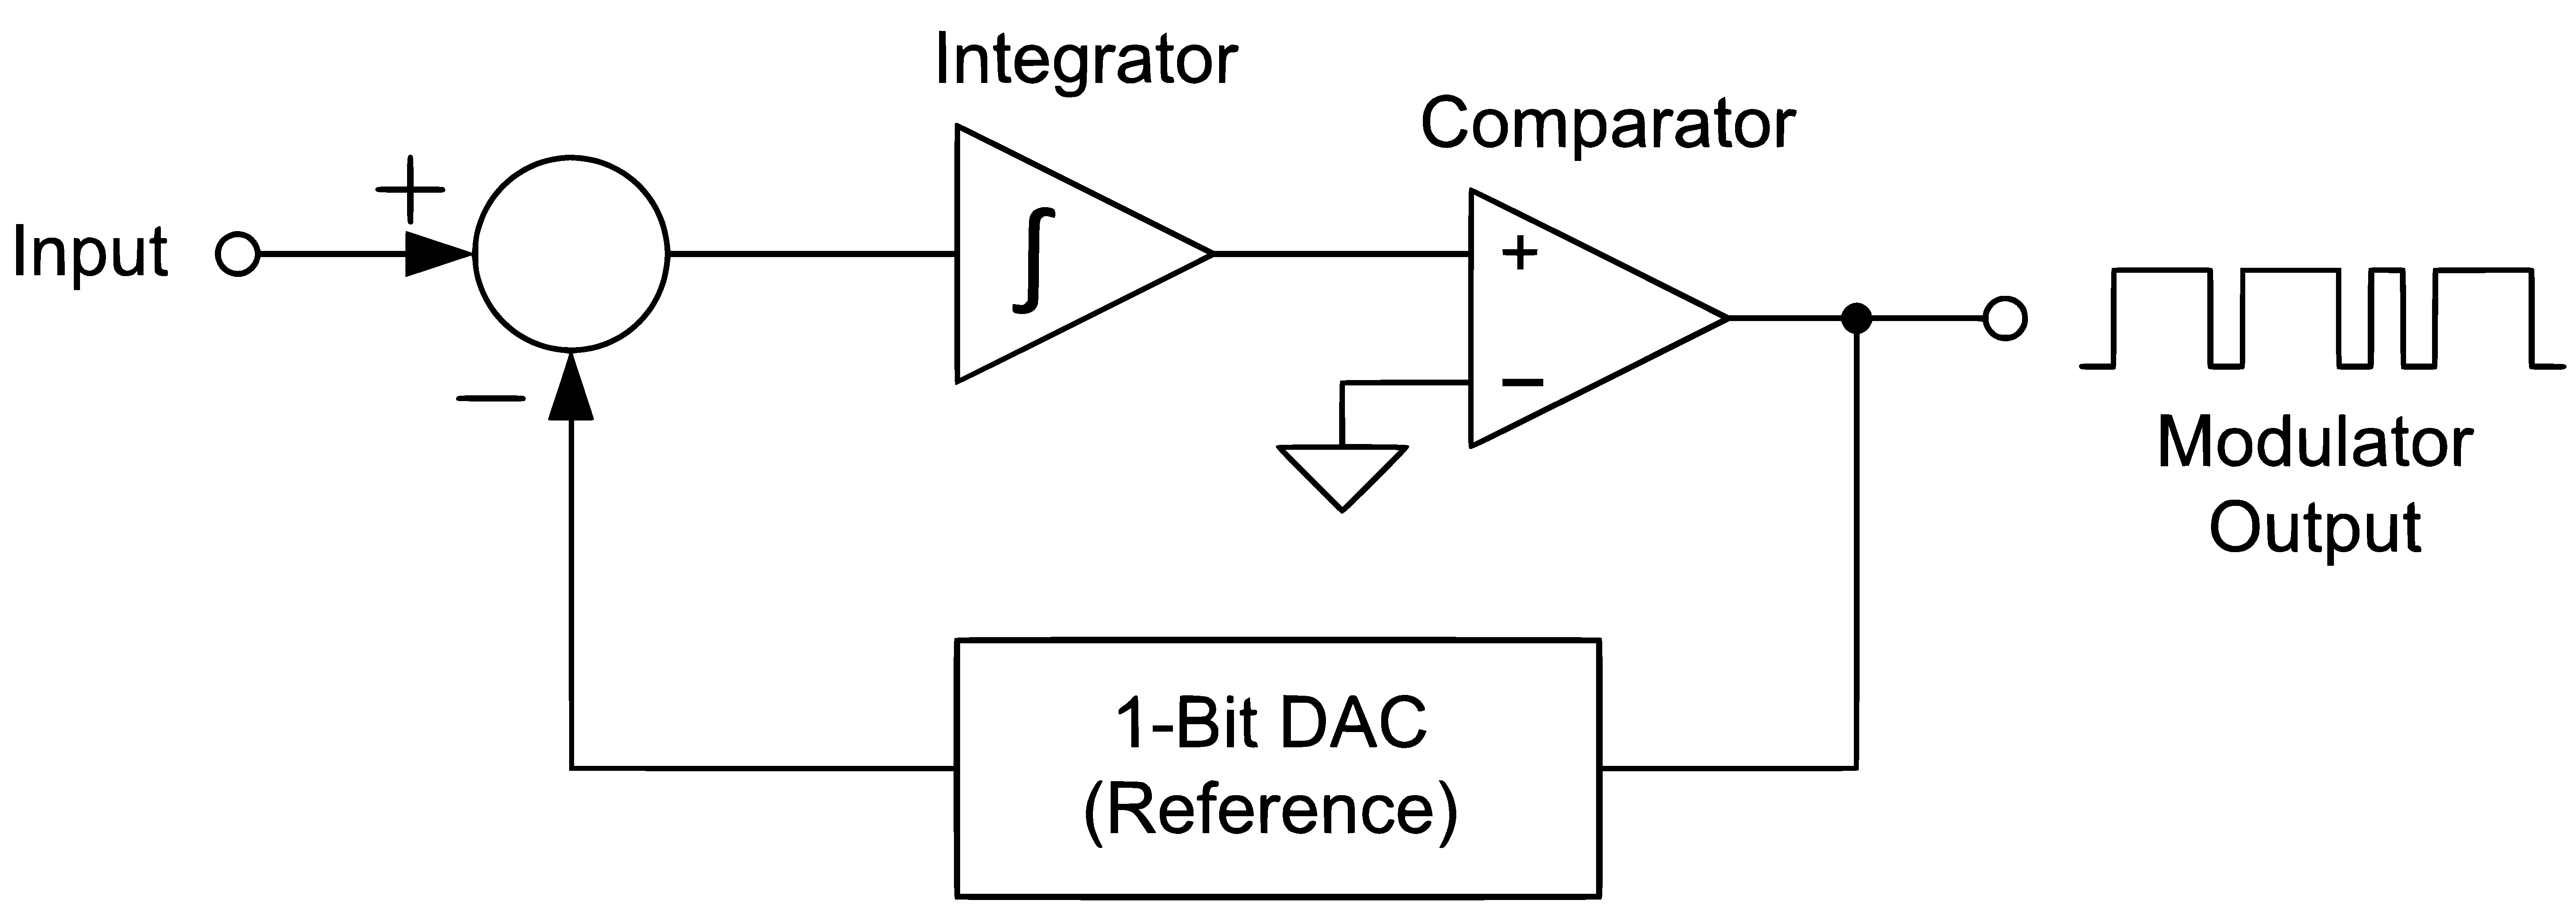
\includegraphics[width=0.7\textwidth]{eps/sigma-delta.eps}
    \caption{Schématique symbolique d'un modulateur \Sigma{}-\Delta{}.
    Le signal d'entrée \og{}Input\fg{} est de nature analogique.
    Le circuit agit en boucle fermée pour compenser la différence entre entrée et sortie.}
    \label{fig:sigmaDelta}
\end{figure}

\subsection{Amplificateur de classe D}
\label{sec:classeD}
La famille des amplificateurs contient plusieurs divisions --- dénommées \og{}classes\fg{} --- selon la nature du signal en sortie.
Par exemples :
les amplificateurs de classe A sortent une tension sinusoïdale amplifiée sur les deux crêtes ;
les amplificateurs de classe B ne laissent sortir qu'une seule crête amplifiée du sinus.

Les amplificateurs de classe D imposent des tensions aux rails d'alimentation du circuit.
C'est du tout ou rien.
Ils sont composés de transistor MOSFET.
Les transistors MOSFET sont les favoris de l'électronique de basse puissance.
Ils peuvent travailler à haute fréquence (plusieurs dizaines de kHz) et leur résistance à la conduction en saturation \og{}R\textsubscript{DS,ON}\fg{} est très faible (une centaine de m\Omega{} dans les basses puissances)~\cite{irf2017mosfet}.
Cette propriété donne tout son intérêt à l'amplificateur de classe D.
En ouvrant ou fermant complètement les transistors pour les faire fonctionner dans leur zone saturée, on minimise la résistance de conduction.
Sachant que la perte en conduction est dû à l'effet joule, et que la puissance de l'effet joule se formule comme $P=RI^2$~\cite{griffiths1999introduction}.
Lorsque $R$, la résistance du transistor est minimale, la puissance $P$ perdue à la conduction est minimisée pour une courant $I$ donné~\cite{sente2017elec}.
Le principe de l'amplificateur de classe D est présenté visuellement à la figure~\ref{fig:classeD}.
Un filtre LC peut-être placé à la suite de l'étage d'amplification pour lisser le courant et la tension~\cite{wildi2005electrotech}.
Dans notre réalisation, nous considérons que le bobinage du haut-parleur lissera le courant et nous ne placerons pas d'inductance discrète.

\begin{figure}[htbp]
    \centering
    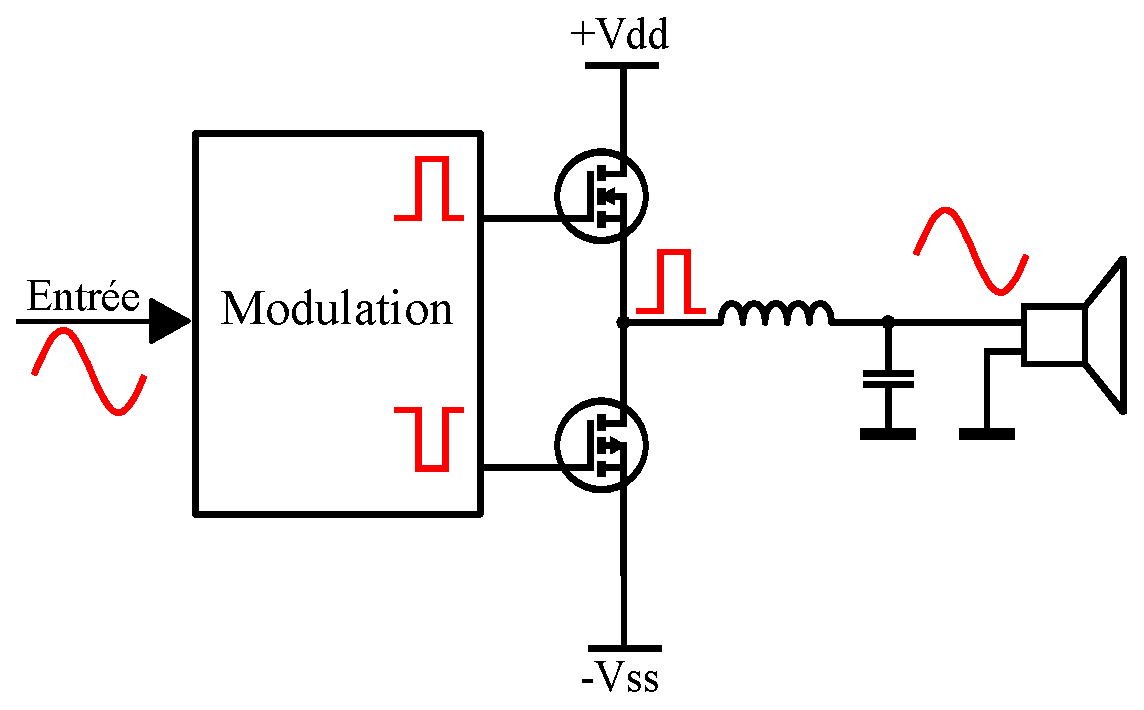
\includegraphics[width=0.5\textwidth]{eps/classe-d.eps}
    \caption{Schématique du principe de l'amplificateur de classe D.
             Le signal d'entré analogique est modulé en commande de commutation de
             transistor de puissance.
             Le signal amplifié se trouve à l'état $+\text{Vdd}$ ou $-\text{Vss}$
             uniquement.
             Ce signal est ensuite lissé au travers d'un filtre LC pour retrouver
             des tensions intermédiaires.}
    \label{fig:classeD}
\end{figure}


%%%%%%%%%%%%%%%%%%%%%%%%%%%%%%
\section{Filtrage des signaux}
À la section~\ref{sec:hypothese}, il a été considéré que la fréquence du signal d'entrée varie entre \num{20} et \SI{22000}{\hertz}.
Pour se débarasser des fréquences hors de cette bande, \textit{i.e.} du bruit, nous filtrons le signal.
Il existe 2 familles de filtre selon les composants électroniques utilisés :
\begin{itemize}
    \item\textbf{Les filtre passifs} sont réalisés avec des composants passifs uniquement : principalement des résistances, des inductances et des condensateurs.
        Leur gain ne peut dépasser 1.
    \item\textbf{Les filtres actifs} contiennent des composants actifs : des transistors et des amplificateurs opérationnels.
        Ils peuvent amener de la puissance et donc un gain supérieur à 1.
\end{itemize}
La réponse fréquentielle d'un filtre se définit comme l'évolution d'amplitude et de phase d'un signal le traversant en fonction de la fréquence.
Le diagramme de Bode est une représentation de la réponse fréquentielle.
Nous nous intéressons uniquement aux filtres passes-bas et passe-haut étant donné que ce sont les seuls utilisés dans le circuit.
\begin{itemize}
    \item\textbf{Les filtre passe-bas} laissent passer toutes les fréquences depuis
        la fréquence nulle jusqu'à la fréquence de coupure et atténue toutes les
        fréquences supérieures qui lui sont supérieures.
    \item\textbf{Les filtre passe-haut} atténuent toutes les fréquences depuis la
        fréquence nulle jusqu'à la fréquence de coupure et laisse passer toutes
        celles qui lui sont supérieures.
\end{itemize}
Pour rappel, la fréquence de coupure d'un filtre, notée par la suite $f_c$, est la fréquence limite de fonctionnement utile de ce filtre.
Elle est défini à \SI{-3}{\decibel}, là où le signal perd la moitié de sa puissance.
Ainsi, nous définissions deux fréquences de coupures :
\begin{itemize}
    \item la $f_c$ du filtre passe-bas à \SI{22000}{\hertz}
    \item la $f_c$ du filtre passe-haut à \SI{20}{\hertz}
\end{itemize}
La combinaison de ces deux filtres en série nous permettra d'obtenir une filtre passe-bande.


%%%%%%%%%%%%%%%%%%%%%%%%%%%%%%%%
\section{Schématique du circuit}
Depuis une vue d'ensemble, le circuit que nous avons réalisé peut se diviser en trois parties : les filtres d'entrées et de pré-amplification ; le comparateur Sigma-Delta, et l'étage de puissance.
Cette section présente successivement chacune de ces parties.
Les schémas complets sont disponibles aux annexes.

\subsection{Filtres d'entrées}
La figure~\ref{fig:schemaPreAmpli} présente les parties de pré-amplification et de filtrage reçues au cours.
Le trajet emprunté par le signal est le suivant : le signal analogique arrive sur la pin \texttt{ININV\underline{A}}.
La résistance \texttt{R15} n'existe pas.
Étant donné la nécessité d'un filtre passe-haut, un condensateur est ajouté entre les pins \texttt{ININV\underline{A}} et \texttt{ININV\underline{B}}.
C'est par là que le signal se dirige.
Une fois le condensateur traversé, le signal rencontre la résistance \texttt{R14} puis arrive à l'entrée inverseuse d'un amplificateur opérationnel avec rétro-action (\texttt{C18} et \texttt{R13}).
La sortie de cet AOP, dénommée par \texttt{OUTINV}, renvoie un signal filtré.

On peut apercevoir que le montage de filtrage et de pré-amplification n'est autre qu'une simple combinaison d'une implémentation élémentaire d'un filtre passe-haut et filtre passe-bas.
\begin{figure}[!ht]
    \centering
    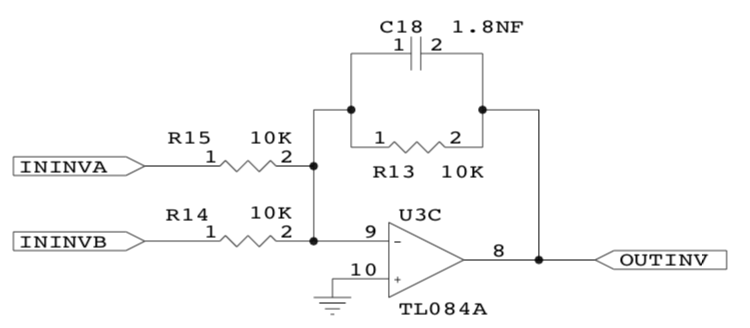
\includegraphics[width=0.6\textwidth]{image/schematique-all.jpg}
    \caption{Circuit schématique du filtre d'entrée et de préamplification de la partie
             Sigma-Delta.}
    \label{fig:schemaPreAmpli}
\end{figure}

Afin de mieux distinguer le montage, les figures~\ref{fig:filtreLowpass} et \ref{fig:filtreHighpass} présentent respectivement le circuit d'un filtre élémentaire passe-bas et d'un filtre passe-haut :

\begin{minipage}[t]{.45\textwidth}
    \centering
    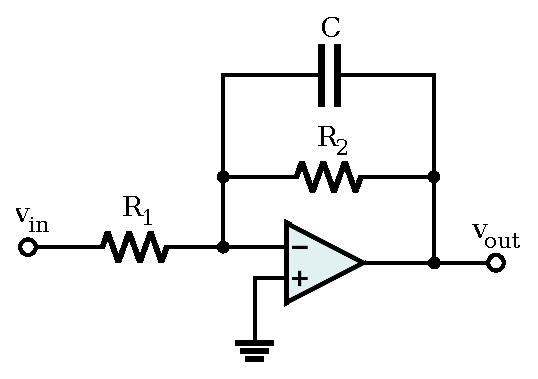
\includegraphics[height=110pt]{eps/active-lowpass-filter-rc.eps}
    \captionof{figure}{Implémentation élémentaire d'un filtre actif passe-bas déséquilibré.}
    \label{fig:filtreLowpass}
\end{minipage} \hfill
\begin{minipage}[t]{.45\textwidth}
    \centering
    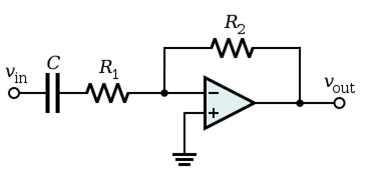
\includegraphics[width=\textwidth]{image/active-highpass-filter-rc.png}
    \captionof{figure}{Implémentation élémentaire d'un filtre actif passe-haut déséquilibré.}
    \label{fig:filtreHighpass}
\end{minipage}

\subsection{Alimentation}
La figure~\ref{fig:alimDecouplage} présente le circuit de découplage de l'alimentation.
Cela ne présente que peux d'intérêt mais est énoncé pour montrer son existence.

\begin{figure}[!ht]
	\centering
	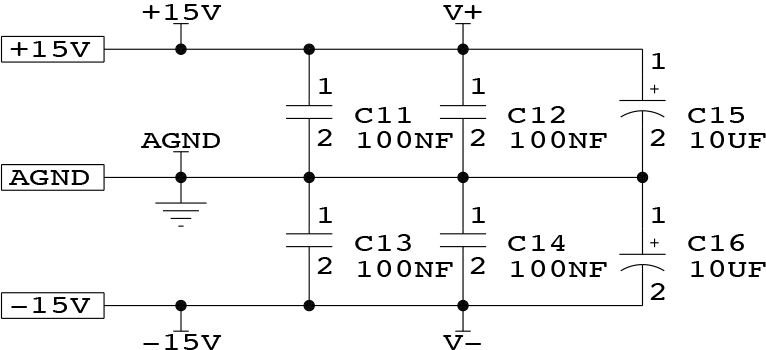
\includegraphics[width=6cm]{image/sch-alim.png}
	\caption{Schématique du circuit découplage d'alimentation.}
	\label{fig:alimDecouplage}
\end{figure}

\subsection{Comparateur Sigma-Delta}
Avant de détailler le développent de la modulation sigma-delta, rappelons le principe de 2 composants essentiels à sa mise en oeuvre : 
\begin{itemize}
\item \noindent\textbf{L'intégrateur pur} présenté à la figure~\ref{fig:IntegPur} ci-dessous, est un montage électronique dont le signal de sortie $V_{S}$ correspond à l'intégrale du signal d'entrée $V_{E}$.
L'équation suivante traduit la relation d'intégration entre sortie et entrée : 
\begin{equation}
    V_{S} = -\frac{1}{RC}\int V_{E}\,dt
\end{equation}
\begin{figure}[!ht]
	\centering
	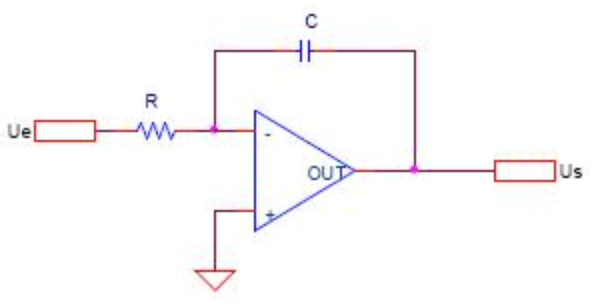
\includegraphics[width=6cm]{image/integrateur.png}
	\caption{Schématique d'un montage intégrateur pur.}
	\label{fig:IntegPur}
\end{figure}

\item \noindent\textbf{Le comparateur} présenté à la figure~\ref{fig:Comparateur} ci-dessous, n'est ni plus ni moins qu'un amplificateur opérationnel dont le fonctionnement est le suivant : si la tension appliquée sur l'entrée non inverseuse $V_{1}$ dépasse la tension appliquée sur l'entrée inverseuse $V_{2}$, la sortie se retrouve à 1.
Dans le cas contraire, la sortie se trouve à 0.
Le figure~\ref{fig:Comparateur_Graphe} présente la sortie du comparateur (signal vert) en fonction de ses deux entrées.
L'équation suivante traduit cette relation entre l'entrée et la sortie du comparateur : 
\begin{align}
\begin{cases}
 V_{S} = V^{+} &\text{si } V_{1} > V_{2} \\
 V_{S} = 0     &\text{si } V_{1} < V_{2}
\end{cases}
\end{align}
\begin{figure}[!ht]
	\centering
	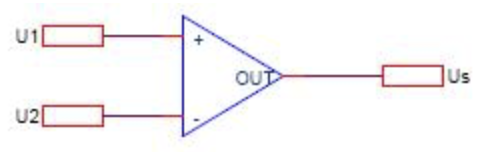
\includegraphics[width=6cm]{image/comparateur.png}
	\caption{Schématique d'un comparateur.}
	\label{fig:Comparateur}
	\centering
	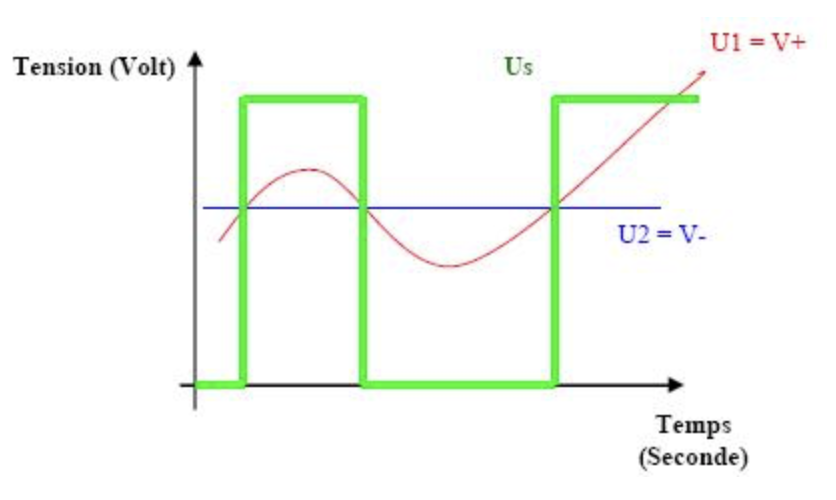
\includegraphics[width=6cm]{image/Graphe_Comparateur.png}
	\caption{Schématique d'un comparateur.}
	\label{fig:Comparateur_Graphe}
\end{figure}
\end{itemize}
La figure~\ref{fig:sch-ctrl} présente la partie logique du circuit, celle qui analyse le signal analogique et le module en commande d'ouverture de transistor.
Le signal rentre par la connection \texttt{OUTINV} provenant des filtres d'entrées de pré-amplifications.
À ce signal est ajouté la sortie actuelle du comparateur \texttt{VMLI} pour différentier l'erreur.
Comme la sortie du comparateur est bi-state en 0 ou \SI{15}{\volt}, sa valeur moyenne en régime permanent serait de \SI{7.5}{\volt}.
C'est vers cette valeur \og{}neutre\fg{} que nous voulons tendre si aucun signal n'est amené à l'entrée du comparateur.
Pour ce faire, nous connectons à la jonction une piste à \SI{-15}{\volt} reliée par une résistance deux fois plus grande que celles des autres connections.
Cette résistance deux fois plus grande laisse passer la quantité de courant nécessaire à amener la jonction à \SI{7.5}{\volt} au repos.

Le premier AOP \texttt{U3A} agit tel un intégrateur et intègre la différence entre la mesure et la consigne.
Le second AOP \texttt{U5B} réagit en trigger de Schmitt et fixe sa sortie en bi-state \SI{\pm15}{\volt} suivant que l'erreur entre la mesure et la consigne soit positive ou négative.

\begin{figure}[!ht]
	\centering
	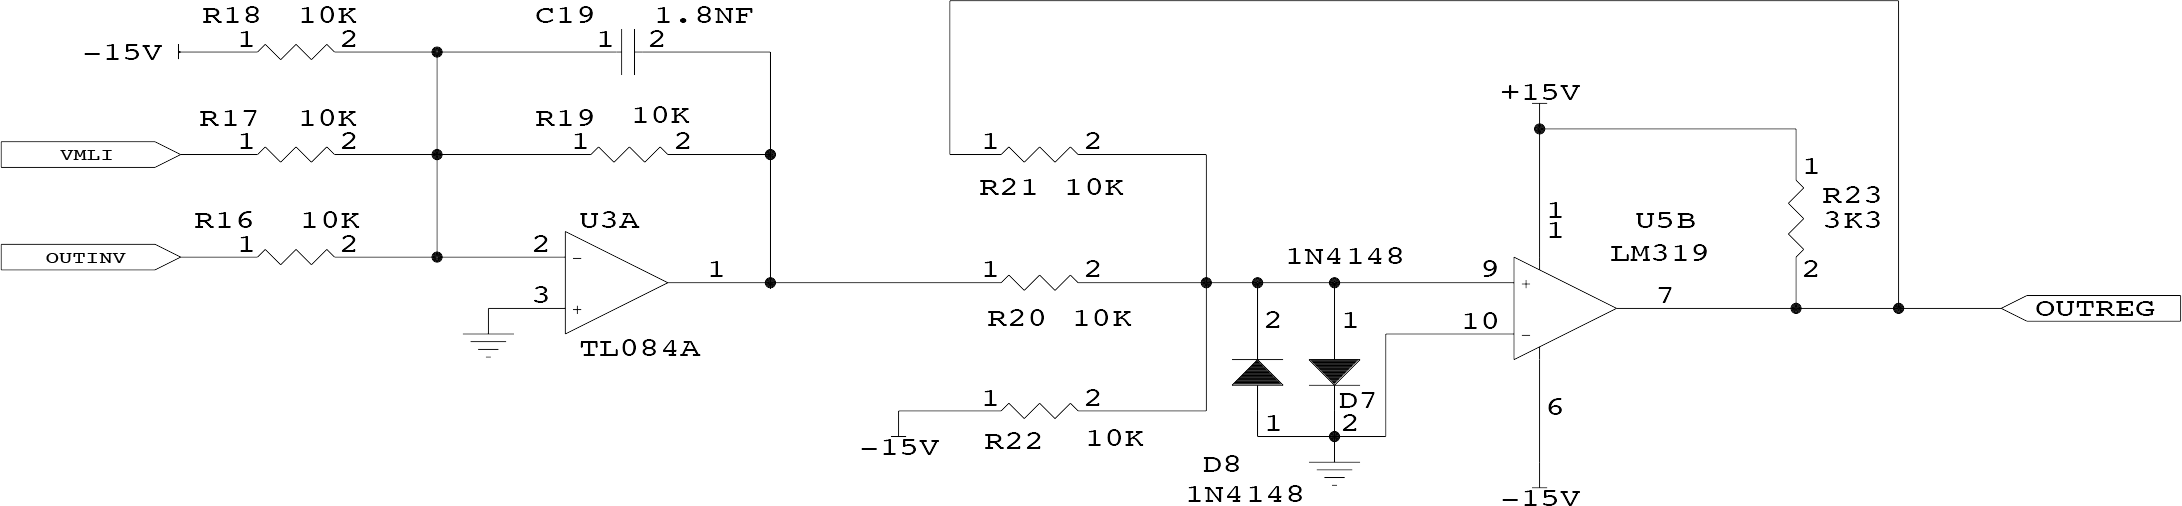
\includegraphics[width=\textwidth]{image/sch-ctrl.png}
	\caption{Schématique du circuit de comparaison Sigma-Delta.}
	\label{fig:sch-ctrl}
\end{figure}

\subsection{Étage de puissance}
La commande d'ouverture des transistors arrive par \texttt{CMDMOS}.
Ce signal est dédoublé et l'une des sortie est inversée afin de contrôler les deux transistors alternativement.
Le circuit intégré \texttt{L6385} se charge de commander les grilles des transistors en y plaçant une tension adaptée grâce à son condensateur de bootstrap.
Le haut-parleur, charge RL dans le circuit, est connecté à la junction entre le transistor MOS supérieur et l'inférieur au jumper 1.
Pour une raison de facilité, la source de tension \SI{24}{\volt} située au jumper 5 est relié à la même source que le driver MOS.

\begin{figure}[!ht]
	\centering
	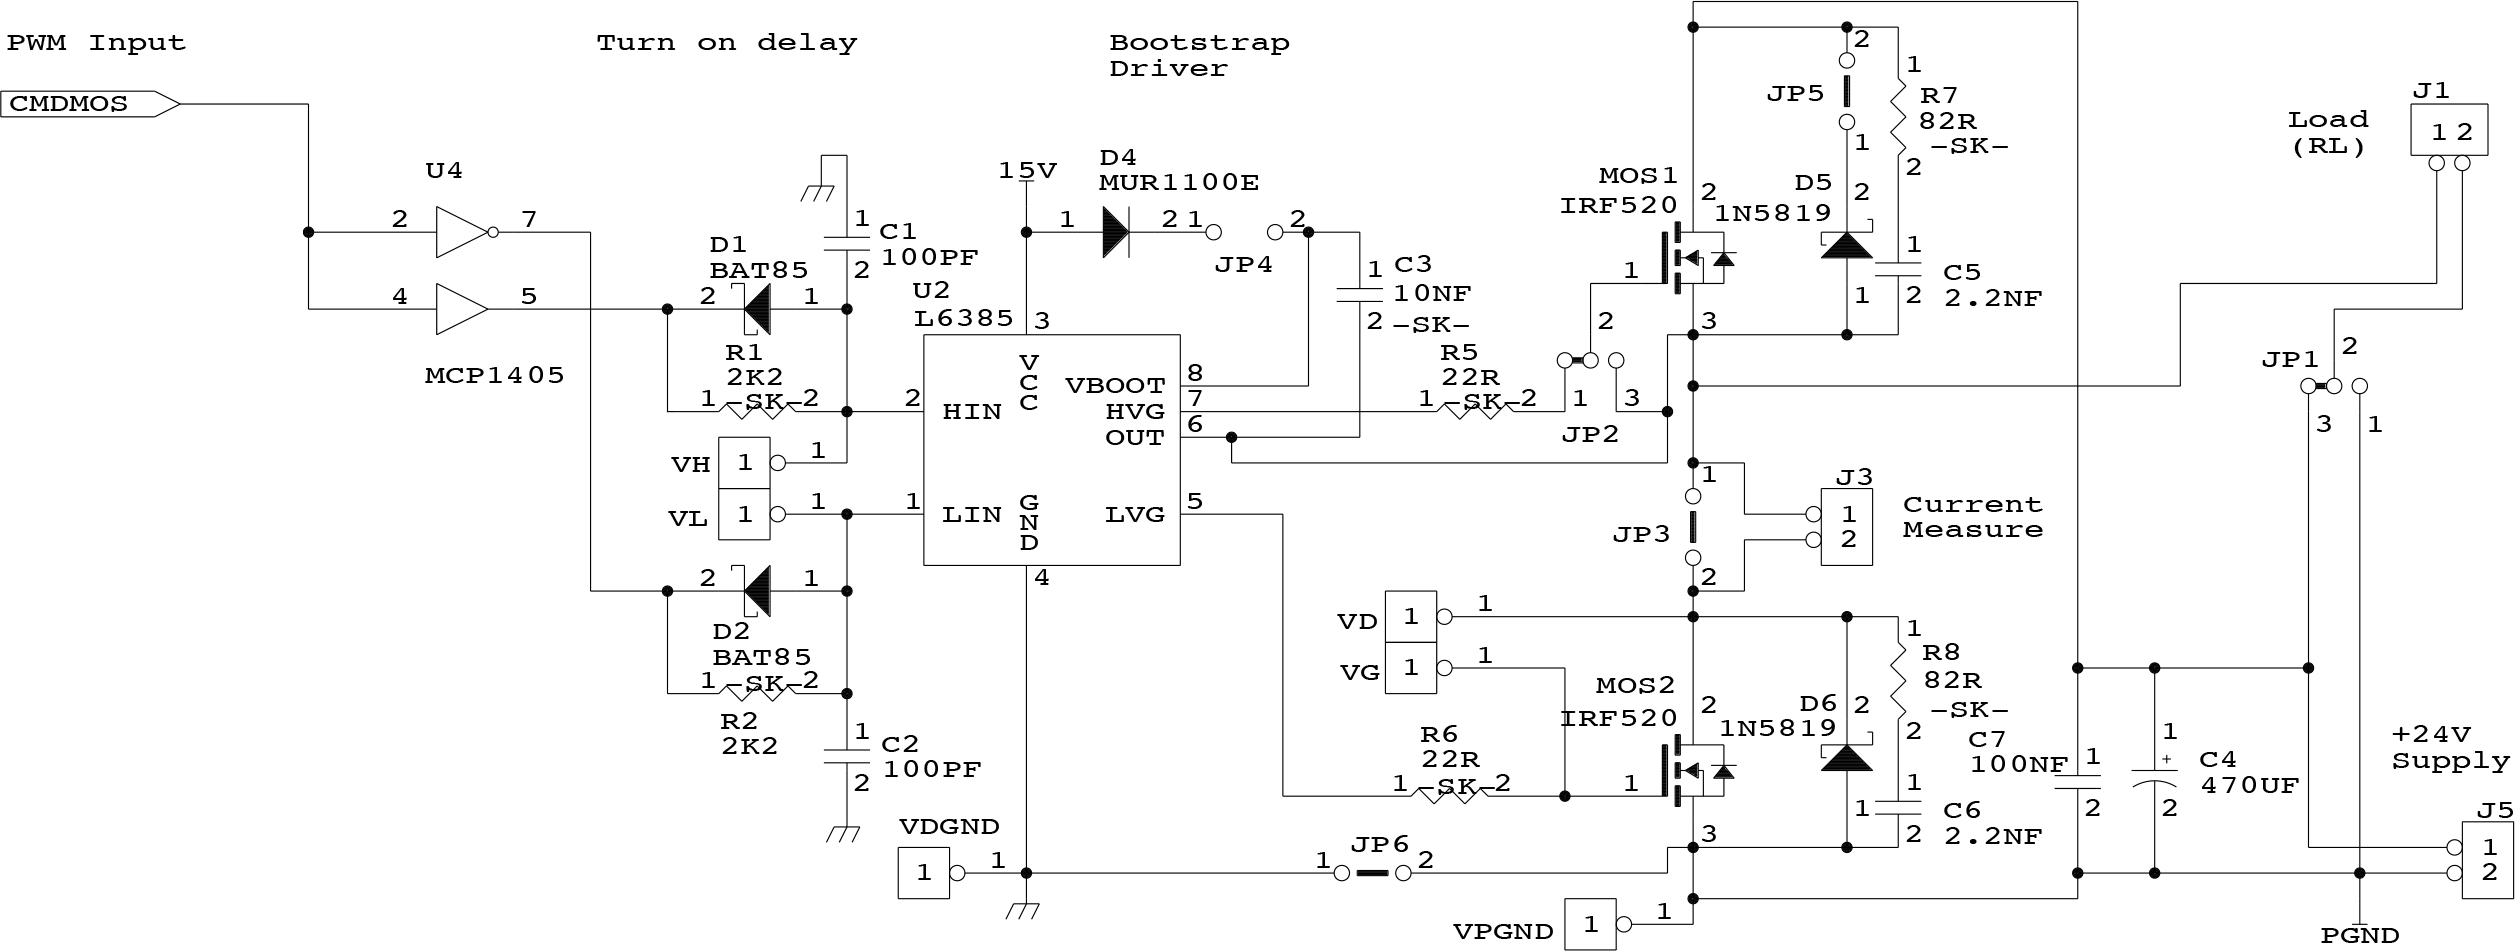
\includegraphics[width=\textwidth]{image/sch-mos.png}
	\caption{Schématique de l'étage de puissance, un circuit d'amplification par transistor
			 MOS.}
	\label{fig:sch-mos}
\end{figure}

%%%%%%%%%%%%%%%%%%%%%%%%%
\section{Dimensionnement}
Cette section aborde nos choix de composant dans la réalisation des filtres et du temps d'intégration du Sigma-Delta.
Ces choix sont accompagnés de calcules appuyant nos décisions.

\subsection{Filtres d'entrées}
\label{sec:filtrePreAmpli}
Pour dimensionner les composants électroniques (résistances et condensateurs) des deux filtres de l'amplificateur classe D, nous avons procédé comme suit :

\textit{N.B.} Se référer aux figures~\ref{fig:filtreLowpass} et \ref{fig:filtreHighpass} pour les notations.
Les éléments R1 et C1 sont connectés entre l'entrée et la borne négative de l'AOP, les éléments R2 et C2 sont connectés à la rétro-action de cet AOP.

\noindent\textbf{Pour le filtre passe-bas} : durant le laboratoire, nous avons commencé par
dimensionner le filtre passe-bas.
La fréquence de coupure doit se trouver aux environ de \SI{20}{\kilo\hertz}.
Prendre les formules théoriques permettant de calculer la fréquence de coupure
et le gain de l'amplificateur :
\begin{gather}
    f_c = \frac{1}{2\pi R_2 C_2} \\
    A_v = -\frac{R_2}{R_1}
    \intertext{Poser comme hypothèse que nous souhaitons un gain unitaire.
			   Cela signifie que la valeur de la résistance R1 est égale à la valeur
			   de la résistance R2.}
    A_v = - \frac{R_2}{R_1} = -1
	\intertext{Fixer une valeur standard pour R2 et réécrire la formule permettant
			   de trouver la valeur de C2.
			   Nous avons pris une valeur standard de \SI{8.2}{\kilo\Omega} pour la résistance R2.}
    R_1 = R_2 = \SI{8.2}{\kilo\Omega} \\
    C_2 = \frac{1}{2\pi R_2 f_c}
    \intertext{Cherchant une valeur la plus standardisée possible pour le condensateur
    		   C2, nous devons ajuster la valeur de la fréquence de coupure dans la
		   	   formule donnée précédemment.
			   Ceci nous conduit à ajuster la fréquence de coupure à \SI{19400}{\hertz}.}
    C_2 = \frac{1}{2\pi\;8200\times19400} = \SI{1}{\nano\farad}
\end{gather}

\noindent\textbf{Pour le filtre passe-haut} : la fréquence de coupure doit se trouver aux environ
de 20 Hz.
Nous connaissons déjà les valeurs standards des deux résistances R1 et R2 ainsi que
du condensateur C2.
Il nous reste donc à calculer la valeur standard du condensateur C1.
Prendre la formule théorique permettant de calculer la fréquence de coupure
\begin{gather}
    f_c = \frac{1}{2\pi R_2 C_1}
	\intertext{Réécrire la formule permettant de calculer la valeur standard de C1}
    C_1 = \frac{1}{2\pi R_2 f_c}
	\intertext{Connaissant la valeur de R2, nous trouvons la valeur de C1 en ajustant
			   la valeur de la fréquence de coupure. Nous trouvons finalement une
			   fréquence de coupure de 18 Hz.}
    C_1 = \frac{1}{2\pi R_2 f_c} = \frac{1}{2\pi\,8200\times18} = \SI{1}{\micro\farad}
\end{gather}
Le tableau~\ref{tab:recapFiltres} reprend les valeurs calculées pour les filtres passe-bas et passe-haut :
\begin{table}[htbp]
    \centering
    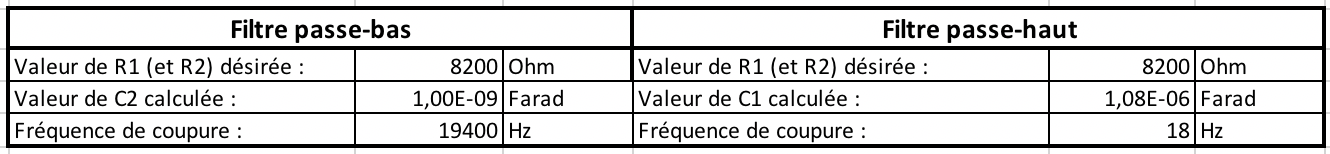
\includegraphics[scale=0.65]{image/tableau-filtres.jpg}
    \caption{Tableau récapitulatif des valeurs calculées pour les filtres de l'amplificateur classe D.}
    \label{tab:recapFiltres}
\end{table}


%%%%%%%%%%%%%%%%%%%%%%%%%%%%
\section{Analyse du circuit}
Après que les éléments aient été dimensionnée, nous avons opté pour analyser le circuit en le faisant fonctionner en régime normal et en prenant des mesures en différents points.
Ces mesures sont toujours, sauf si cité explicitement, en tension par rapport à la masse, elle même mise à la terre.

\subsection{Problèmes rencontrés}
\label{sec:problems}
Dés le premier branchement de la carte en tension symétrique \pm\SI{25}{\volt}DC,
nous avons observé un appel de courant de \SI{200}{\milli\ampere} sur le circuit.
Cette valeur était le maximum parametré sur l'alimentation de laboratoire à notre portée.
Ce courant est trop élevé pour un amplificateur au repos, c.-à-d. sans signal d'entrée.
Il n'y a nul doute qu'un problème de connexion existe sur la carte.

Pour cerner le problème, nous avons connecté un ohmmètre entre les bornes d'alimentation : positive-négative, positive-neutre, neutre-négative.
À ces bornes nous avons mesuré respectivement une résistance de : \SI{33}{\Omega}, \SI{9}{\kilo\Omega} et \SI{9}{\kilo\Omega}.
C'est désormais déterminé et mesuré, il existe un défaut de connexion entre la borne positive et le neutre.

Une analyse bloc-par-bloc a permis de déterminer que le problème était le circuit intégré \texttt{TC4428}, un double inverseur présentant un courant de fuite de \SI{100}{\milli\ampere} pour une tension d'alimentation de seulement \SI{4.3}{\volt};
ce qui est déraisonnable et en opposition avec la fiche technique du produit.
Nous en avons déduit que le composant était détruit.

Après avoir remplacé le circuit intégré \texttt{TC4428}, nous avons observé que la résistance entre la borne d'alimentation positive et le neutre passait de \SI{33}{\Omega} à \SI{200}{\Omega}, ce qui n'est toujours pas acceptable.
Nous avons remplacé un second circuit intégré douteux, le \verb|L6385E|, et la résistance est passée de \SI{200}{\Omega} à \SI{19}{\kilo\Omega}; ce qui est désormais raisonnable.
Tout cela démontre que deux des circuits imprimés ont été détruits.
Nous ne savons pas déterminer l'instant auquel cela s'est produit.

Un autre problème rencontré a été le court-circuit à chaque mesure.
Cela nous a semblé surprenant mais à chaque fois que la sonde passive de l'oscilloscope avec une résistance interne de \SI{10}{\mega\Omega} touchait une piste, l'alimentation de laboratoire se bloquait à la limite de courant.
Secouer la carte entrainait également ce phénomène.
Nous avons remplacé les soudures direct fil-à-carte en soudant des connecteurs femelles dans les jonctions mais cela n'a pas réglé le soucis.
Néanmoins cela l'a rendu plus reproductible car désormais nous pouvions dire que c'était dès que le jumper J6 était connecté que le court-circuit apparaissait.
Ce jumper relie la masse du circuit comparateur et celle de l'étage de puissance.
Nous discutons de ce souci par la suite.

\subsection{Filtres d'entrées}
Voulant savoir si les valeurs théoriques calculées au point~\ref{sec:filtrePreAmpli}
conduisent à des filtres de fidèle qualité, nous les avons testé.
Nous avons donc tracé, dans le diagramme de Bode de chaque filtre.
Pour ce faire, nous avons utilisé :
\begin{enumerate}
    \item\textbf{Un générateur de signaux} pour générer un signal analogique
        d'amplitude et fréquence connue.
        L'objectif est de faire varier la fréquence du signal d'entrée et d'observer les
        conséquences que cela a sur l'amplitude du signal de sortie.
    \item\textbf{Un oscilloscope} pour mesurer les amplitudes des signaux à l'entrée du
        filtre et à la sortie de ce dernier.
\end{enumerate}

Les tables~\ref{tab:gainFiltresEntrees} reprennent les valeurs mesurées à l'oscilloscope, à savoir tension d'entrée et tension de sortie, ainsi que le calcul du gain en décibel pour chacun des deux filtres :
\begin{table}[!ht]
    \centering
    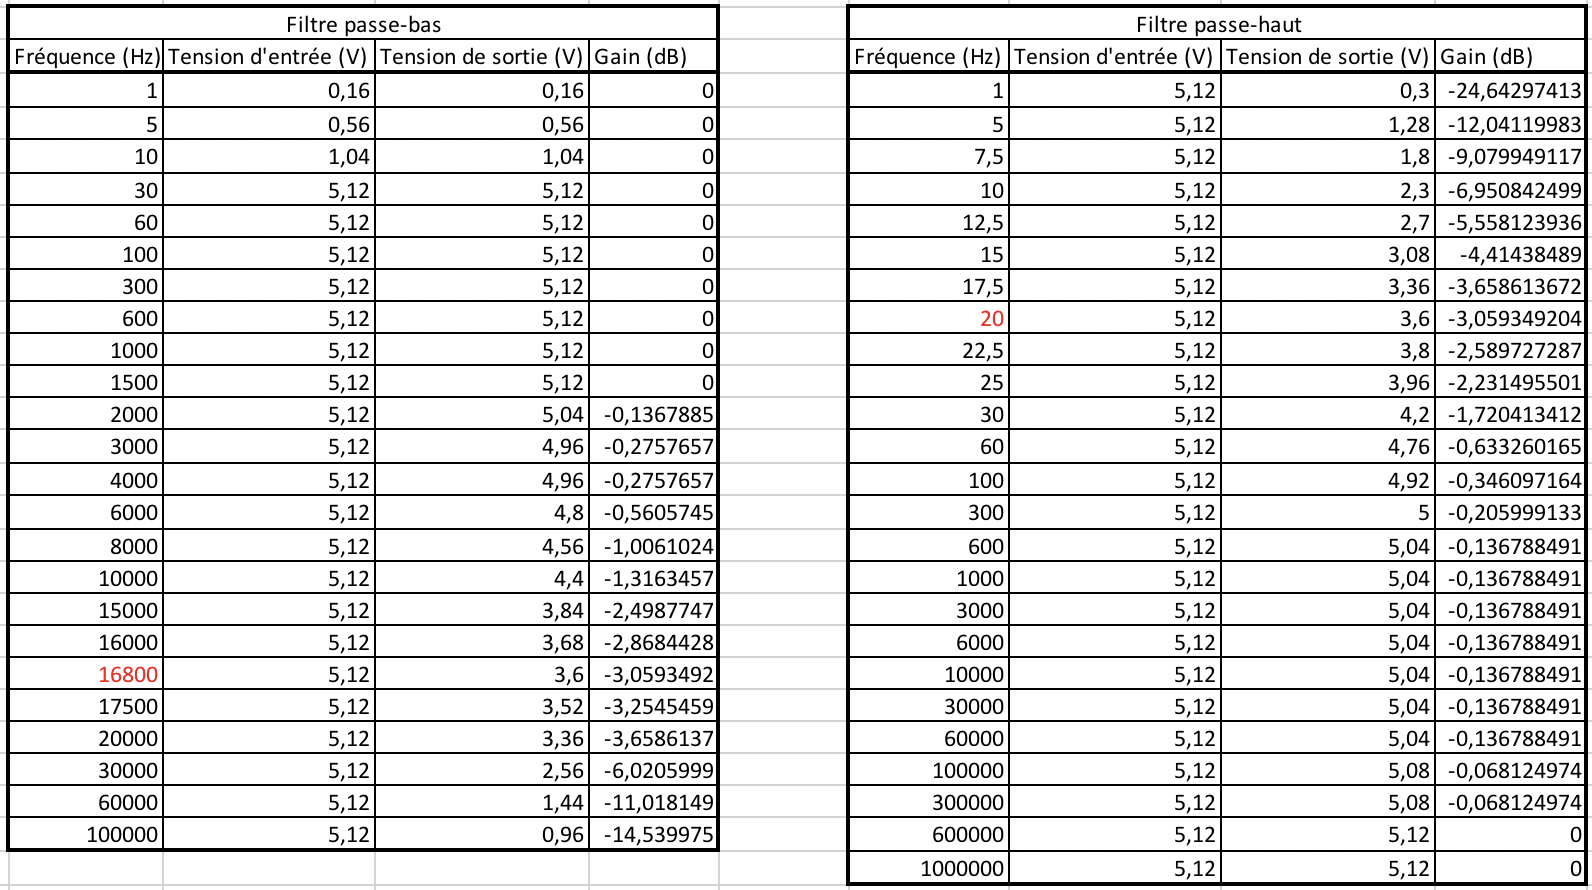
\includegraphics[scale=0.57]{image/resultat-filtres.jpg}
    \caption{Récapitulatif des valeurs mesurées pour les filtres d'entrées.}
    \label{tab:gainFiltresEntrees}
\end{table}

Nous avons réalisé un script Matlab\textregistered{} reprenant toutes les valeurs mesurées et reprises aux tables~\ref{tab:gainFiltresEntrees} afin de représenter la réponse fréquentielle de chacun des filtres dans le diagramme de Bode.
La figure~\ref{fig:resultatRepFreq} présente le résultat obtenu.
Nous pouvons y reconnaitre au gain qu'il s'agit de filtres Butterworth d'ordre 1~\cite{Horowitz:2015aa}.
\begin{figure}[!ht]
    \centering
    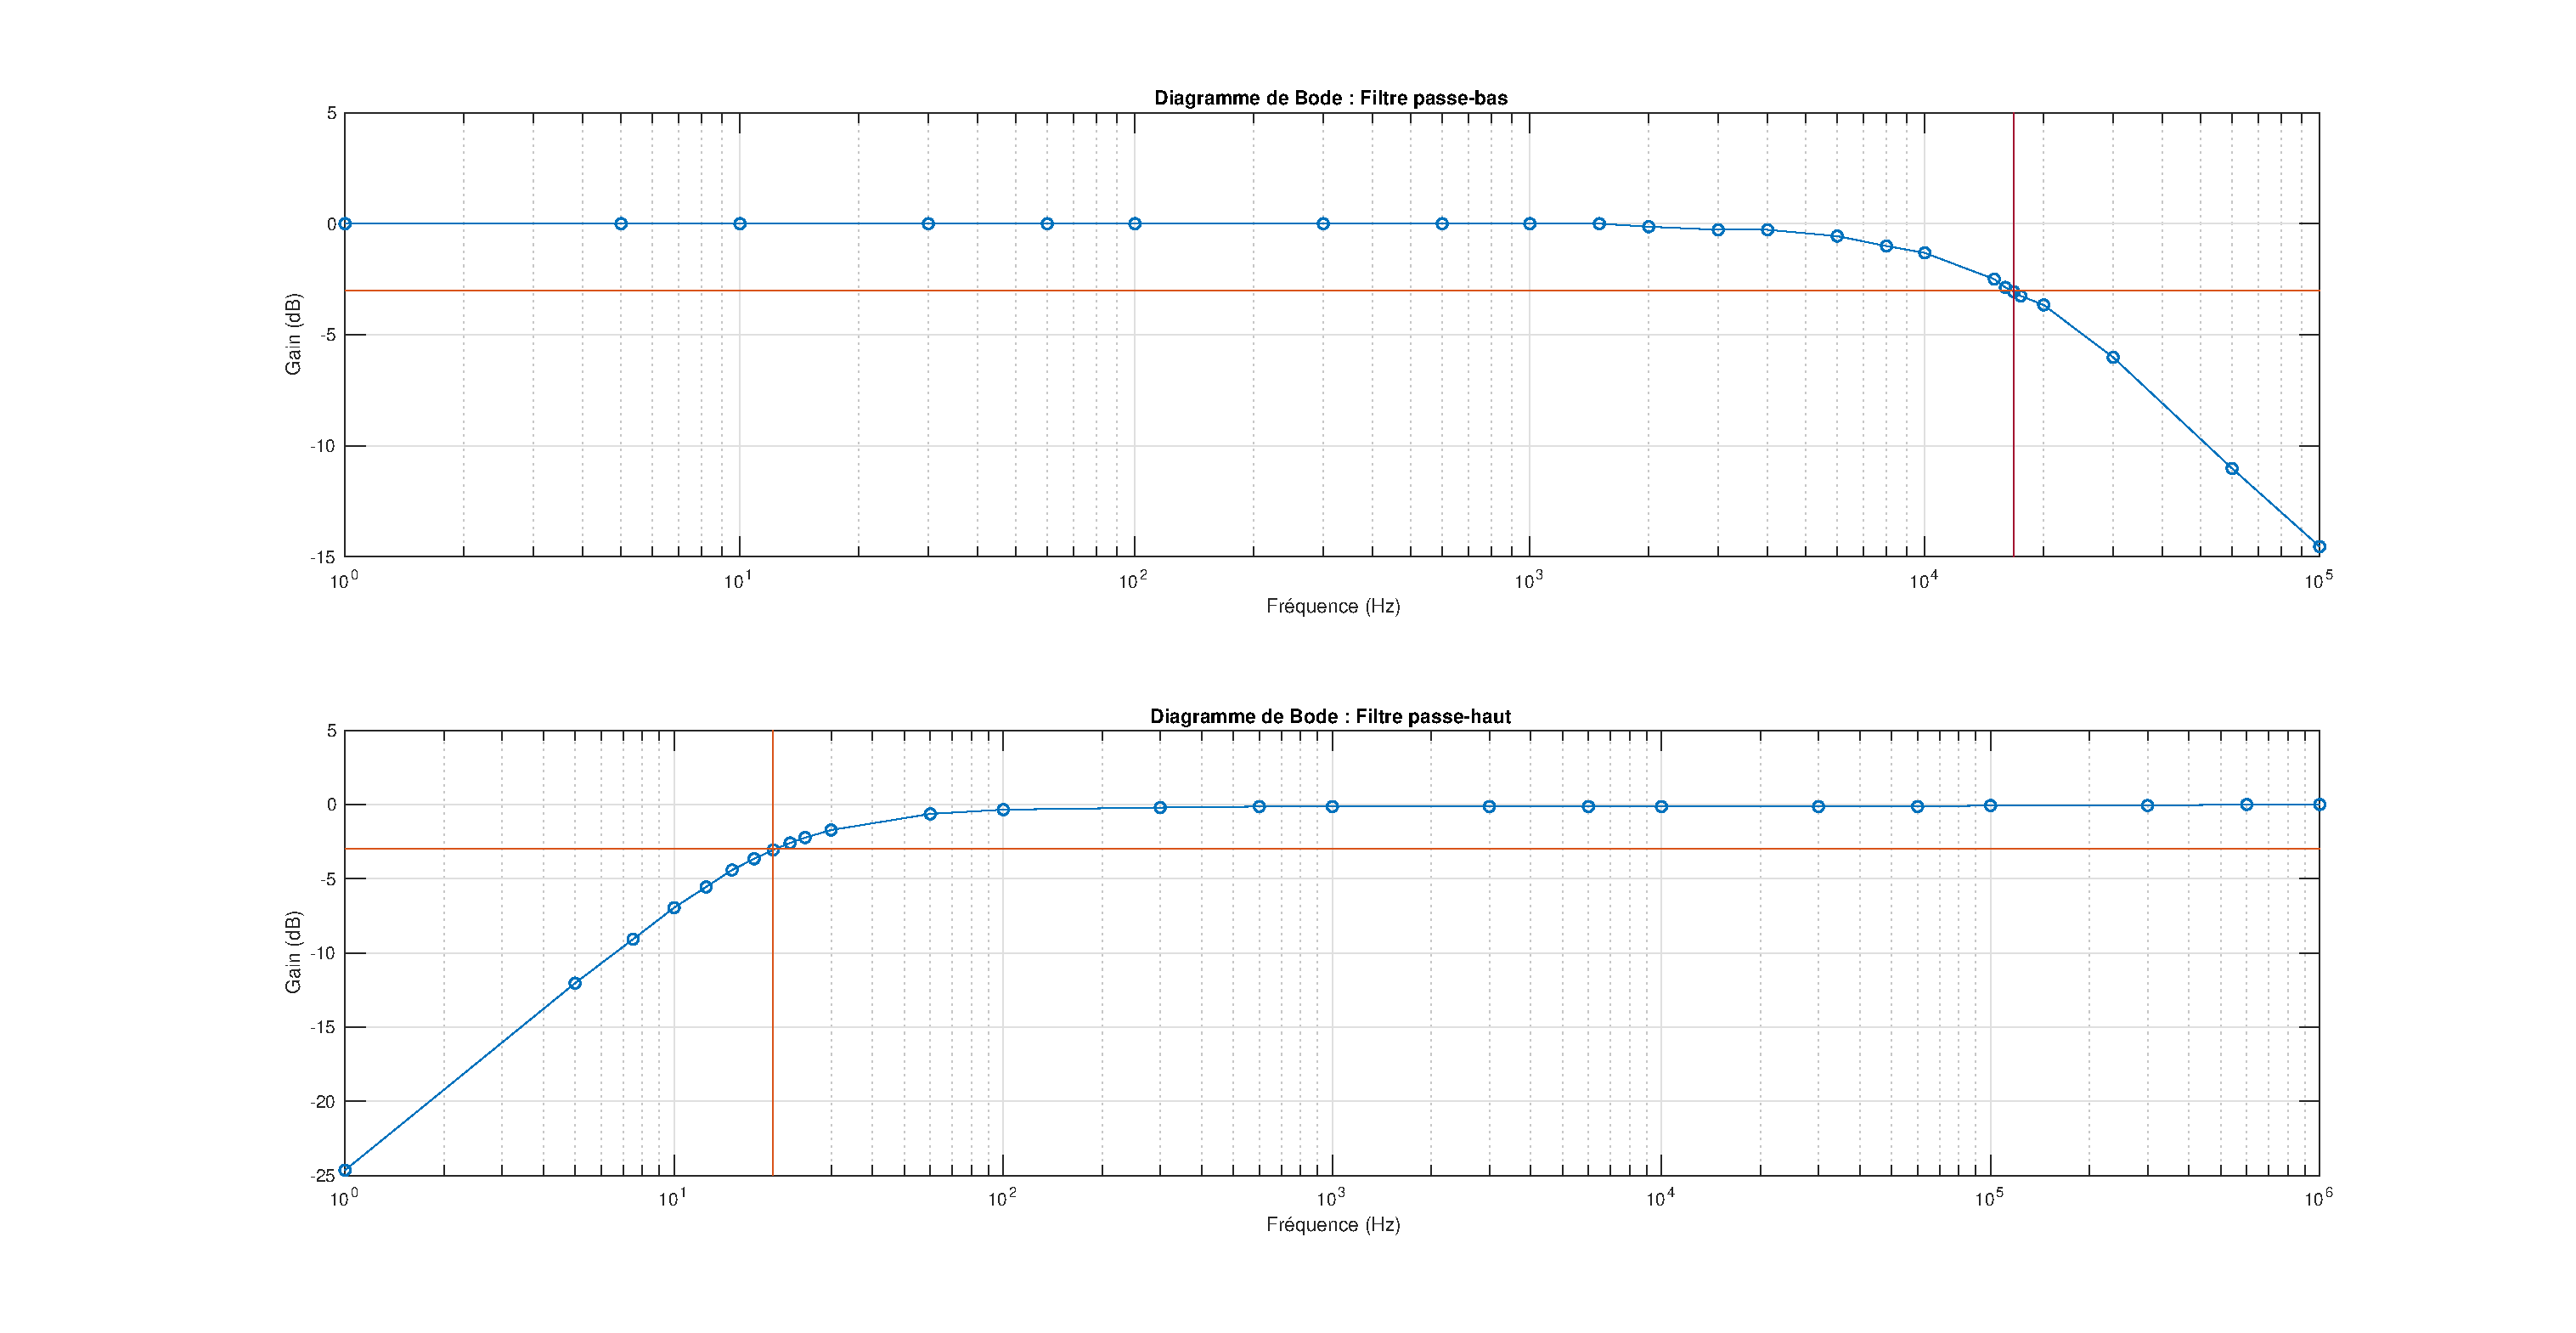
\includegraphics[width=\textwidth]{eps/bode-filtres.eps}
    \caption{Réponse fréquentielle pour les filtres passe-bas
             et passe-haut de l'amplificateur classe D.}
    \label{fig:resultatRepFreq}
\end{figure}

\subsection{Performance du Sigma-Delta}
Malgré que dans son ensemble le circuit ne désire pas fonctionner, nous l'avons dument analyser afin d'en resortir la cause.
Nous abordons dans cette section les mesures effectuées sur la partie Sigma-Delta de la carte.

Avant même d'arrivée dans le comparateur, le signal est filtré par les filtres d'entrées.
La figure~\ref{fig:osci-post-filters} présente la capture d'un signal avant et après son passage au travers du filtre.
Pour une signal sinusoïdale d'amplitude \SI{5}{\volt}pp avec un offtset à \SI{2.5}{\volt} à \SI{1}{\kilo\hertz}, le filtre :
\begin{enumerate}
	\item Retire l'offset (centre le signal autour de \SI{0}{\volt});
	\item Ne modifie pas l'amplitude ni la fréquence;
	\item Retarde la phase de \SI{\pi}{\radian\per\sec}.
\end{enumerate}
Ceci est exactement ce que nous attendons et désirons.

Après filtrage, le circuit arrive dans le comparateur.
La figure~\ref{fig:osci-compar} présente la comparaison entre le signal avant filtrage et l'effet de la retro-action.
Nous constatons que la sortie du comparateur varie à chaque fois que le signal d'entrée atteint sa valeur moyenne.
Avec son duty cycle de \pm50\%, la sortie du comparateur représente bien un signal sinusoïdale.

Ceci nous amènes à regarder le signal \texttt{CMDMOS} à la sortie du Sigma-Delta, la figure~\ref{fig:osci-cmdmos} présente la sortie obtenue pour le signal sinusoïdale présenté précédemment.
Nous y voyons un signal avec une flanc montant adouci et un duty cycle de \num{51.8}\% au moment de la capture.
Encore une fois tout cela semble correcte, nous regardons à la suite au signal dédoublé au travers de l'inverseur \texttt{TC4428}.
Nous y trouvons les commandes d'ouvertes des transistors qui seront transmises au driver.
La figure~\ref{fig:osci-high-low} présente ces commandes.
Elles y apparaissent complémentaires avec chacun cet adoucissement du flanc montant évoqué précédemment.
Cet adoucissement est un effet volontaire introduit avant l'entrée des commandes dans le driver MOS.
Elles ont pour but d'éviter l'ouverture simultanée des deux transistors, ce qui provoquerait un court-circuit.

De l'analyse effectuée jusqu'à présent, le circuit Sigma-Delta semble fonctionner comme désiré pour un signal sinusoïdale.
Nous avons utilisé cette nature de signal car elle est de la même nature que ceux présents dans un signal audio.
Mise à part que leurs fréquences et amplitudes varient.
Nous en décidons que le problème rencontré énoncé dans la sous-section~\ref{sec:problems} ne vient pas du circuit Sigma-Delta, mais de l'étage de puissance à sa suite.

\subsection{Performance de l'étage d'amplification}
Supposant le bon fonctionnement du Sigma-Delta, que nous allons encore cependant vérifier, nous nous sommes mis à prendre des mesures autours du driver MOS et des transistors.
Nous avons voulu vérifier la capacité de l'étage d'amplification à reproduire une tension DC à la sortie de la carte.
Pourquoi une composante DC ?
Parce que sa propriété statique rend l'interprétation des signaux mesurés très aisée.

Premièrement nous devons contourner les filtres d'entrées ; ils contiennent un passe-haut à la fréquence de \SI{20}{\hertz}, bloquant ainsi la composante continue.
Nous en profitons pour évaluer une nouvelle fois le fonctionnement du Sigma-Delta.
Les figures~\ref{fig:scope-2}~\ref{fig:scope-3}~\ref{fig:scope-4} présentent le signal \texttt{CMDMOS} selon la tension DC appliquée en entrée du comparateur.
Nous y distinguons facilement l'échelle et les limites de comparaisons que nous reprenons dans le tableau~\ref{tab:dutyCycleDC}.
\begin{table}[!ht]
	\centering
	\begin{tabular}{|r|r|}
	\hline
	Tension & Duty+ \\
	\hline
	\SI{7}{\volt}  & \num{3.764}\% \\
	\SI{0}{\volt}  & \num{48.80}\% \\
	\SI{-7}{\volt} & \num{96.477}\% \\
	\hline
	\end{tabular}
	\caption{Échelle de modulation MLI du Sigma-Delta pour un signal DC.}
	\label{tab:dutyCycleDC}
\end{table}
Nous sommes étonnés que le duty cycle positif diminue quand la tension DC augmente, mais dans le cas de signaux audios sinusoïdaux, inverser la tension n'influencera guère le son car cette dernière est symétrique autour de 0.

Nous en profitons pour mesurer la fréquence de comparaison du Sigma-Delta.
Elle est de \SI{171.7}{\kilo\hertz}.
C'est bien supérieur au \SI{44}{\kilo\hertz} nécessaire pour échantillonner du son, cela est parfait.

Nous pouvons donc en conclure une fois de plus que le modulateur Sigma-Delta fonctionne comme attendu.
Si nous continuons sur le trajet du signal, nous arrivons à l'inverseur \texttt{TC4428} dédoublant le signal et inversant une sortie.
La figure~\ref{fig:scope-5} présente notre capture entre le signal \texttt{CMDMOS} d'entrée et la commande de transistor supérieur en sortie.
Mise à part une légère modification d'amplitude, nous ne ne constatons pas de problème.

Nous partons donc mesurer les signaux de grilles des transistors supérieur et inférieur à la sortie du driver MOS.
Les figures~\ref{fig:scope-7} et~\ref{fig:scope-8} présentent ces mesures.
Bingo, nous avons trouvé un problème.
La commande du transistor inférieur fonctionne comme attendue : de l'état bas à \SI{0}{\volt}, elle saute à \SI{24.25}{\volt} lorsque \texttt{CMDMOS} tombe à 0.

La commande du transistor supérieur est, par contre, totalement absurde.
C'est une copie de la commande inférieur, avec l'ajout d'un offset de \SI{24}{\volt}.
La commande passe donc de \SI{24}{\volt} quand \texttt{CMDMOS} est haut, à \SI{30}{\volt} quand \texttt{CMDMOS} retombe à 0.
Non seulement ses états sont l'inverse de ce qui est désiré, mais en plus son offet de \SI{24}{\volt} est supérieur à la tension requise d'ouverture des transistors, rendant le transistor supérieur constamment ouvert.

Voilà donc où se trouve le problème entrainant le court-circuit cité à la section~\ref{sec:problems}.
Le transistor supérieur étant constamment ouvert, il amène une tension de la masse virtuelle du circuit de puissance \texttt{VPGND}.
Quand le jumper JP6 est placé, la masse du circuit logique \texttt{VDGND}, qui est directement connecté au neutre de l'alimentation, se retrouve connectée à \texttt{VPGND} où se trouve une tension élevée du au défaut du transistor.
Ceci court-circuitant l'alimentation.

Nous nous sommes dès lors intéressé au driver MOS, et en particulier à au condensateur de bootstrap.
La figure~\ref{fig:scope-10} présente une capture des deux connecteurs du condensateur de bootstrap, sans que ce dernier ne soit connecté.
Le signal \texttt{CMDMOS} est encore présenté pour donner une référence.
On ne remarque que deux signaux malgré que trois sont affichés, les deux connections du condensateur de bootstrap sont indiscernables.
À noter qu'elles sont également un offset de \SI{24.25}{\volt}.
C'est à dire que le condensateur ne voit jamais une différence de tension apparaître entre 
ses broches.
Il est inutile.

Évidement cela n'est pas normal, et après avoir vérifié minutieusement les pistes et soudures de la carte, nous suspectons le driver MOS \texttt{L6385E} d'être non fonctionnel.
Celui même qui avait déjà été remplacé une fois précédemment.

%%%%%%%%%%%%%%%%%%%%%
\section{Conclusion}


%%%%%%%%%%%%%%%%% GROS BAZARD DE FIGURE À LA FIN %%%%%%%%%%%%%%%%%
\pagebreak
\begin{figure}[p]
	\centering
	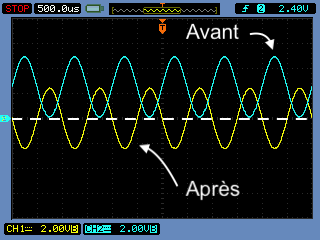
\includegraphics[width=0.65\textwidth]{image/osci-post-filters.png}
	\caption{Capture d'écran d'un oscilloscope affichant le signal capturé avant les
			 filtres d'entrées et le signal capturé après.
			 Au travers du filtre le signal garde son amplitude, est déphasé de
			 \SI{\pi}{\radian\per\second}, et son offset disparait pour se centrer autour
			 de 0.}
	\label{fig:osci-post-filters}
\end{figure}

\begin{figure}[p]
	\centering
	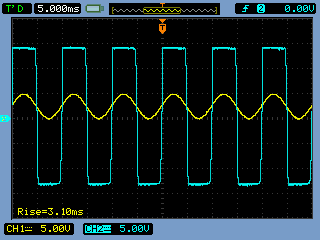
\includegraphics[width=0.65\textwidth]{image/osci-compar.png}
	\caption{Capture d'écran d'un oscilloscope affichant le signal capturé à l'entrée
			 de l'amplificateur (avant filtrage) et la comparaison perçue par le
			 \Sigma{}-\Delta{}.}
	\label{fig:osci-compar}
\end{figure}

\begin{figure}[p]
	\centering
	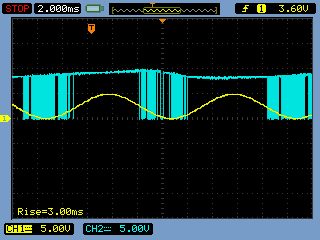
\includegraphics[width=0.65\textwidth]{image/osci-cmdmos.png}
	\caption{Capture d'écran d'un oscilloscope affichant le signal \texttt{CMDMOS}
			 capturé à la sortie du \Sigma{}-\Delta{} pour un signal d'entrée à
			 l'amplificateur sinusoïdale.
			 Le délai d'ouverture à la commande pour éviter la double conduction à
			 l'étage de puissance est la raison de l'affaissement du flanc montant.}
	\label{fig:osci-cmdmos}
\end{figure}

\begin{figure}[p]
	\centering
	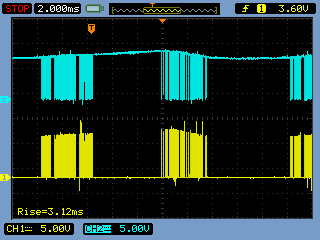
\includegraphics[width=0.65\textwidth]{image/osci-high-low.png}
	\caption{Capture d'écran d'un oscilloscope affichant les signaux de grille des
			 transistors MOS supérieur et inférieur à l'étage d'amplification.
			 Ces commandes sont propres à un signal d'entrée de l'amplificateur
			 sinusoïdale.}
	\label{fig:osci-high-low}
\end{figure}

\begin{figure}[p]
	\centering
	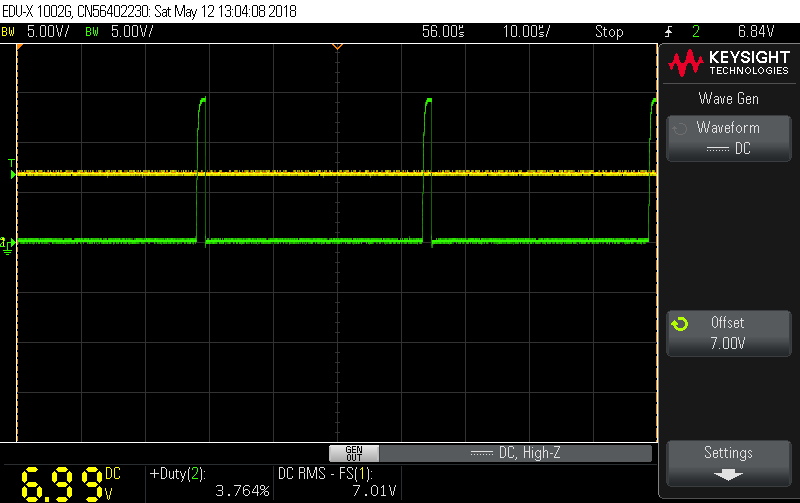
\includegraphics[width=0.65\textwidth]{image/12-05/scope_2.png}
	\caption{Capture d'écran d'un oscilloscope affichant le signal modulé CMDMOS pour une
			 tension d'entrée continue de \SI{7}{\volt}. Le duty cycle est de \num{3.7}\%.}
	\label{fig:scope-2}
\end{figure}

\begin{figure}[p]
	\centering
	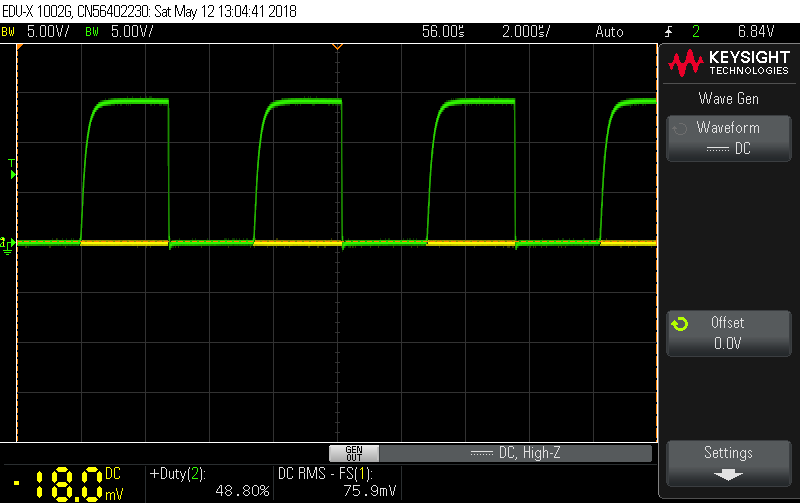
\includegraphics[width=0.65\textwidth]{image/12-05/scope_3.png}
	\caption{Capture d'écran d'un oscilloscope affichant le signal modulé CMDMOS pour une
			 tension d'entrée continue de \SI{0}{\volt}. Le duty cycle est de \num{48.8}\%.}
	\label{fig:scope-3}
\end{figure}

\begin{figure}[p]
	\centering
	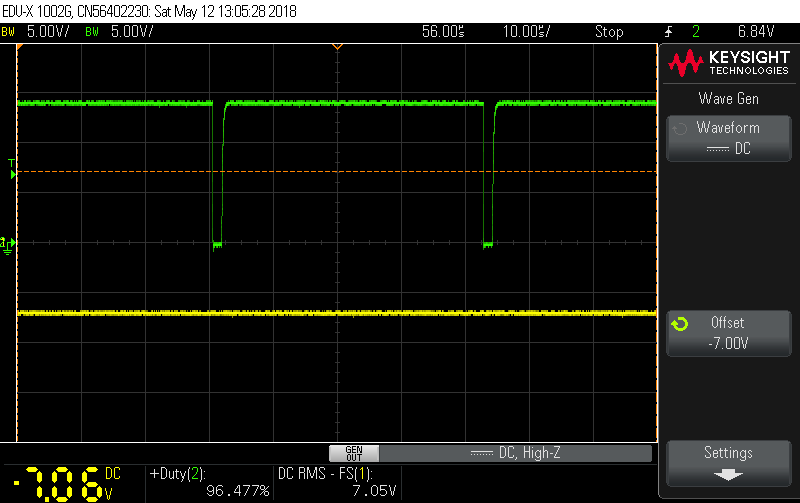
\includegraphics[width=0.65\textwidth]{image/12-05/scope_4.png}
	\caption{Capture d'écran d'un oscilloscope affichant le signal modulé CMDMOS pour une
			 tension d'entrée continue de \SI{-7}{\volt}. Le duty cycle est de \num{96.5}\%.}
	\label{fig:scope-4}
\end{figure}

\begin{figure}[p]
	\centering
	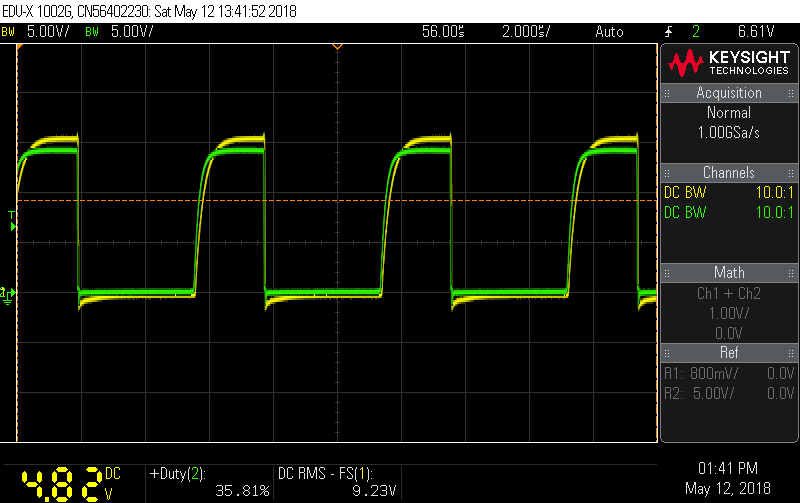
\includegraphics[width=0.65\textwidth]{image/12-05/scope_5.png}
	\caption{Capture d'écran d'un oscilloscope affichant la différence entre le signal
			 modulé CMDMOS et la commande de grille du transistor supérieur.
			 On constate que cette dernière a un léger \og{}skew\fg{}, un décalage
			 temporel et une  variation de l'amplitude.}
	\label{fig:scope-5}
\end{figure}

\begin{figure}[p]
	\centering
	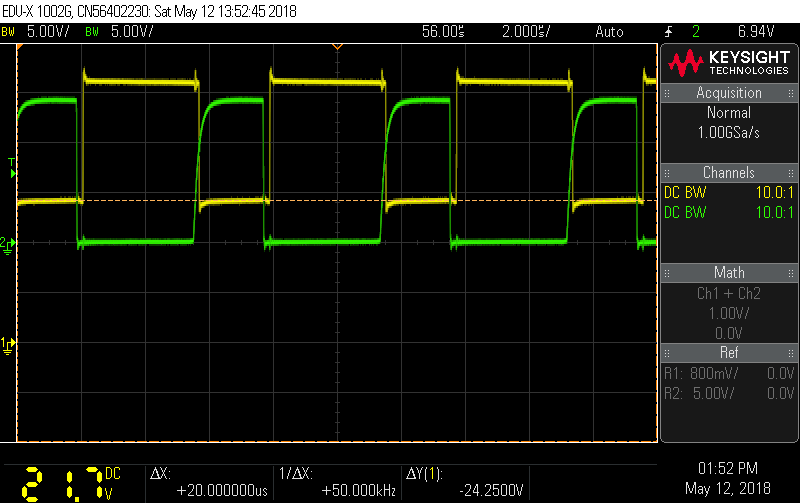
\includegraphics[width=0.65\textwidth]{image/12-05/scope_7.png}
	\caption{Capture d'écran d'un oscilloscope affichant le signal modulé CMDMOS et la
			 commande d'ouverture du transistor supérieur.}
	\label{fig:scope-7}
\end{figure}

\begin{figure}[p]
	\centering
	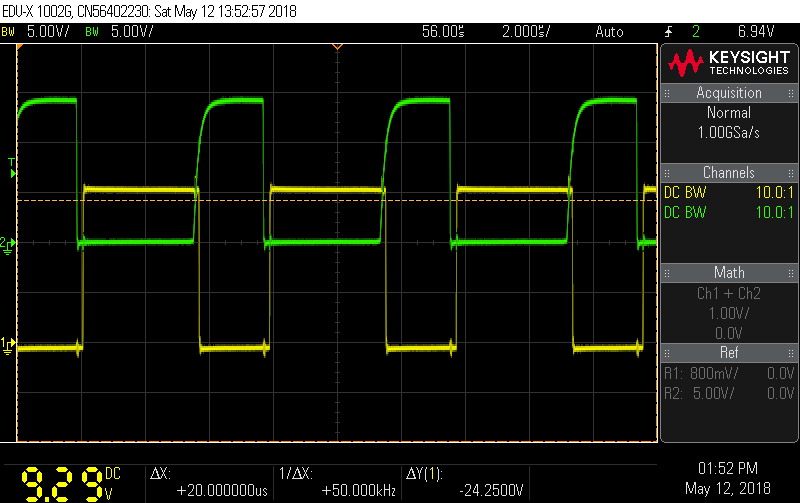
\includegraphics[width=0.65\textwidth]{image/12-05/scope_8.png}
	\caption{Capture d'écran d'un oscilloscope affichant le signal modulé CMDMOS et la
			 commande d'ouverture du transistor inférieur.}
	\label{fig:scope-8}
\end{figure}

\begin{figure}[p]
	\centering
	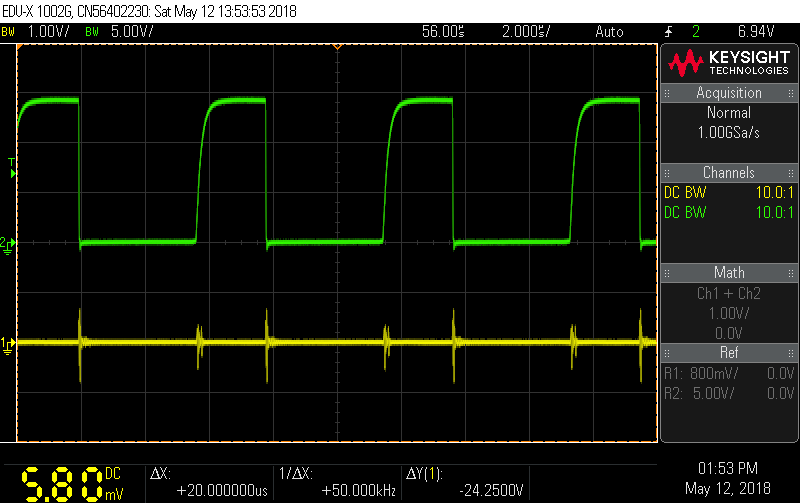
\includegraphics[width=0.65\textwidth]{image/12-05/scope_9.png}
	\caption{Capture d'écran d'un oscilloscope affichant le signal modulé CMDMOS et de
			 la pollution constatable sur la masse.}
	\label{fig:scope-9}
\end{figure}

\begin{figure}[p]
	\centering
	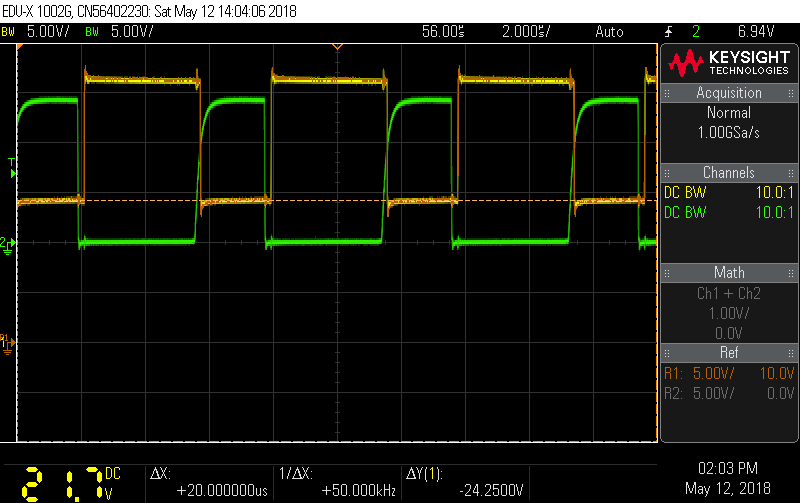
\includegraphics[width=0.65\textwidth]{image/12-05/scope_10.png}
	\caption{Capture d'écran d'un oscilloscope affichant le signal modulé CMDMOS et les
			 connections du condensateur de bootstrap sans que celui-ci ne soit présent.
			 Les deux connections sont mélangés et indiscernable.
			 Le condensateur ne voit pas donc de différence de tension.}
	\label{fig:scope-10}
\end{figure}


%%%%%%%%%%%%%%%%%%
\pagebreak
\section*{Crédits}
\pdfbookmark[1]{Crédits}{sec:credits}
    
\begin{itemize}
\item Figure~\ref{fig:sigmaDelta} provenant de :\\*
Le blog officiel de Texas Instrument :
\url{https://e2e.ti.com/blogs_/archives/b/precisionhub/archive/2015/01/21/delta-sigma-adc-basics-understanding-the-delta-sigma-modulator}

\item Figure~\ref{fig:classeD} provenant de :\\*
Par Yves-Laurent (Travail personnel) [GFDL (\url{http://www.gnu.org/copyleft/fdl.html}),
CC-BY-SA-3.0 (\url{http://creativecommons.org/licenses/by-sa/3.0/})], de Wikimedia Commons

\item Figure~\ref{fig:filtreLowpass} provenant de :\\*
Par Inductiveload (Travail personnel) [Public domain], de Wikimedia Commons

\item Figure~\ref{fig:filtreHighpass} provenant de :\\*
Par Toriicelli (Travail personnel) [Public domain], de Wikimedia Commons
\end{itemize}

%%%%%%%%%%%%%%%%%%%%%%%%%%%%%%%%%%%%%%%%%%%
\pdfbookmark[1]{Références}{sec:references}
\bibliographystyle{unsrt}
\bibliography{ampli-classe-d}

%%%%%%%%%
\appendix
\clearpage
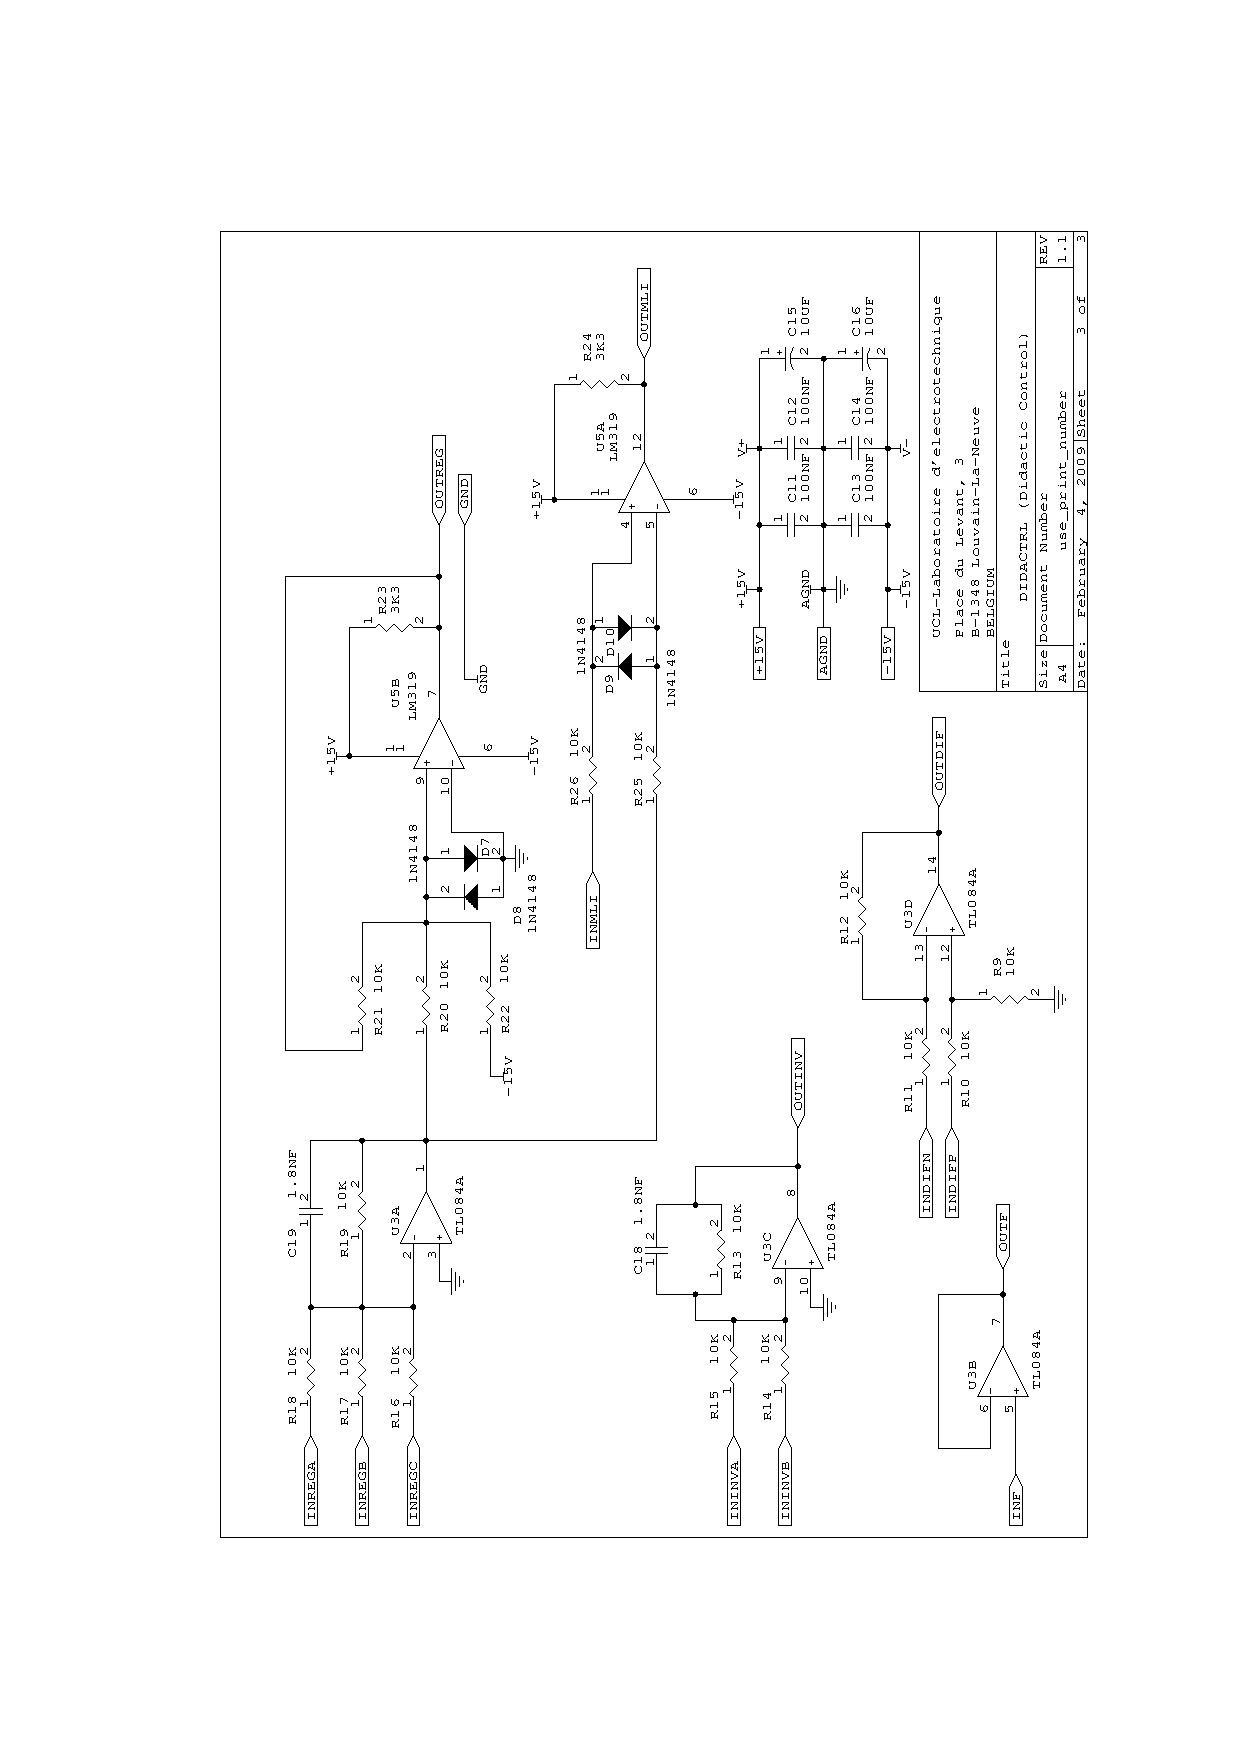
\includepdf[pagecommand=\section{Schéma du circuit DIDACTRL}]{pdf/DIDACTRL.pdf}
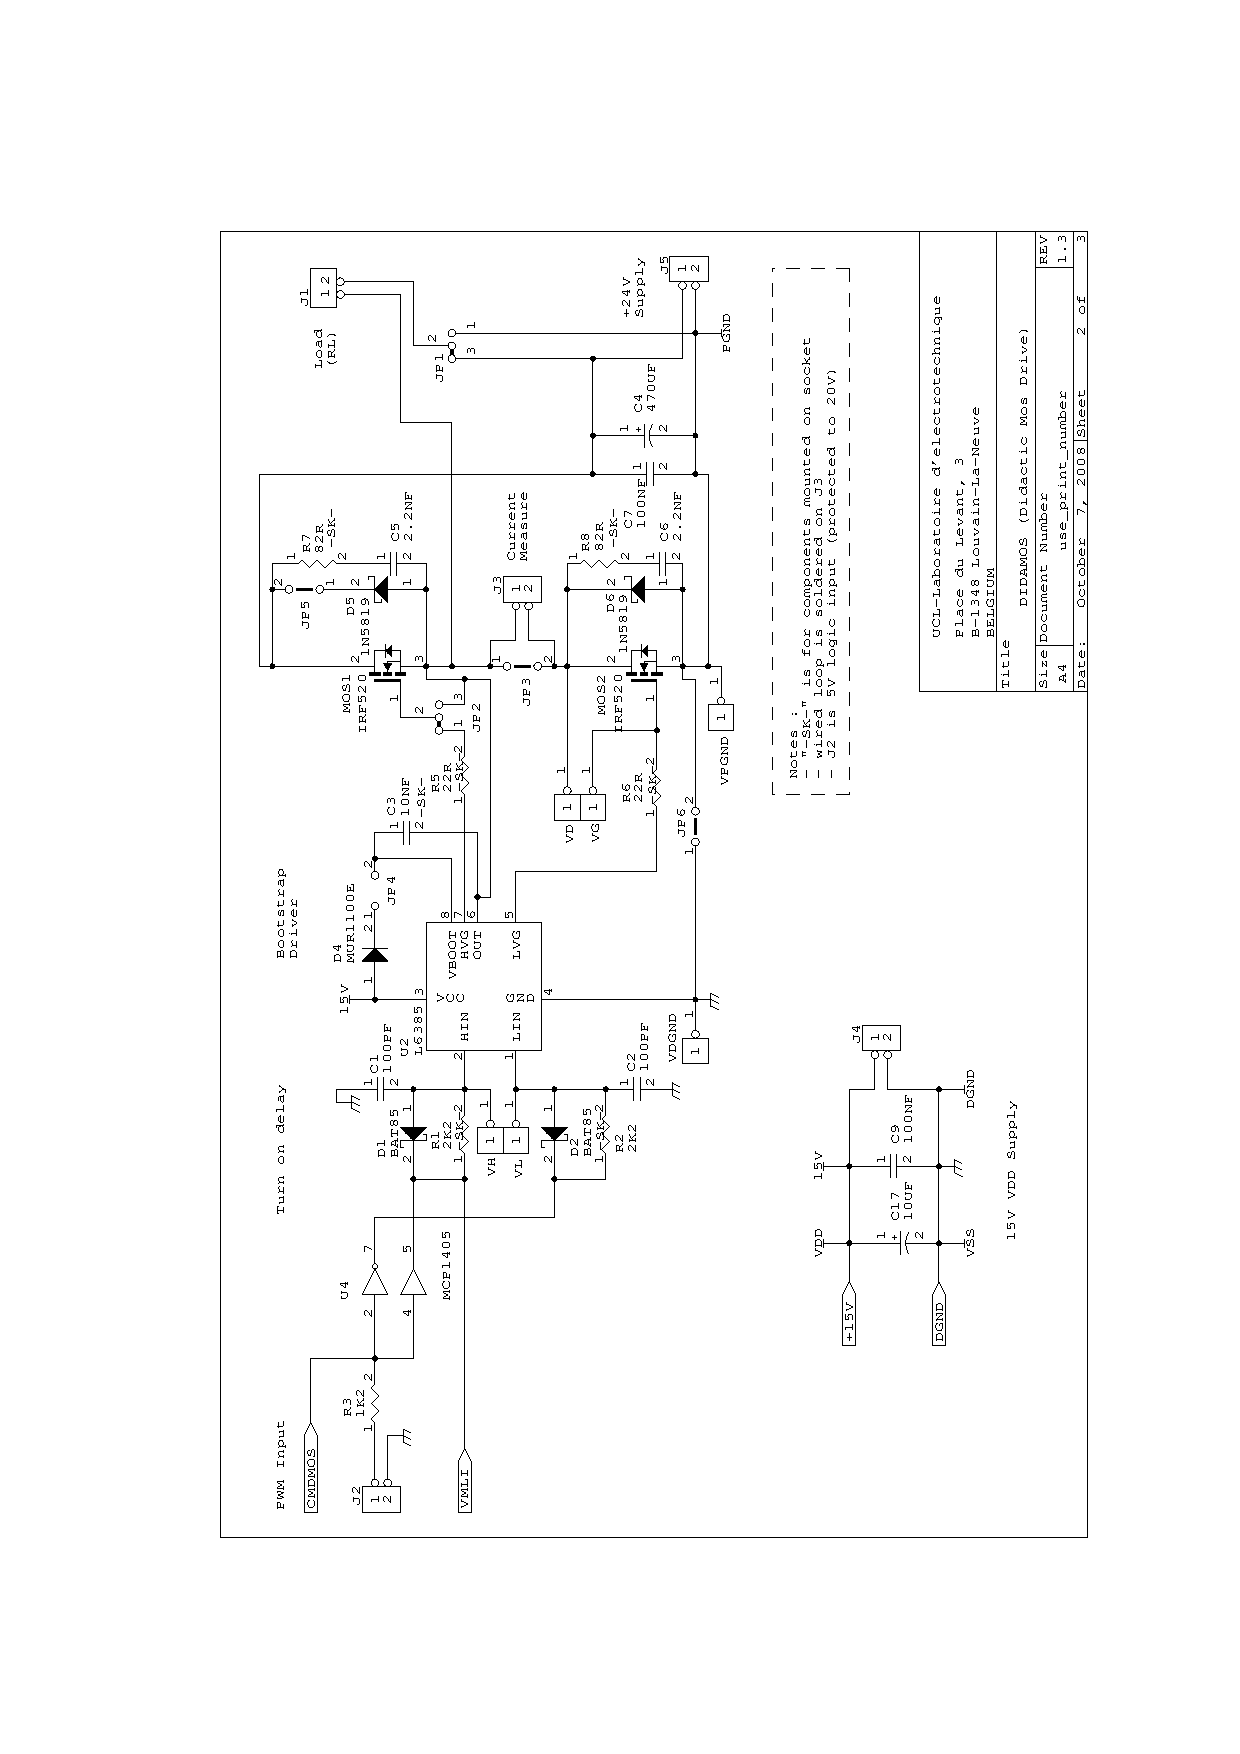
\includepdf[pagecommand=\section{Schéma du circuit DIDAMOS}]{pdf/DIDAMOS.pdf}
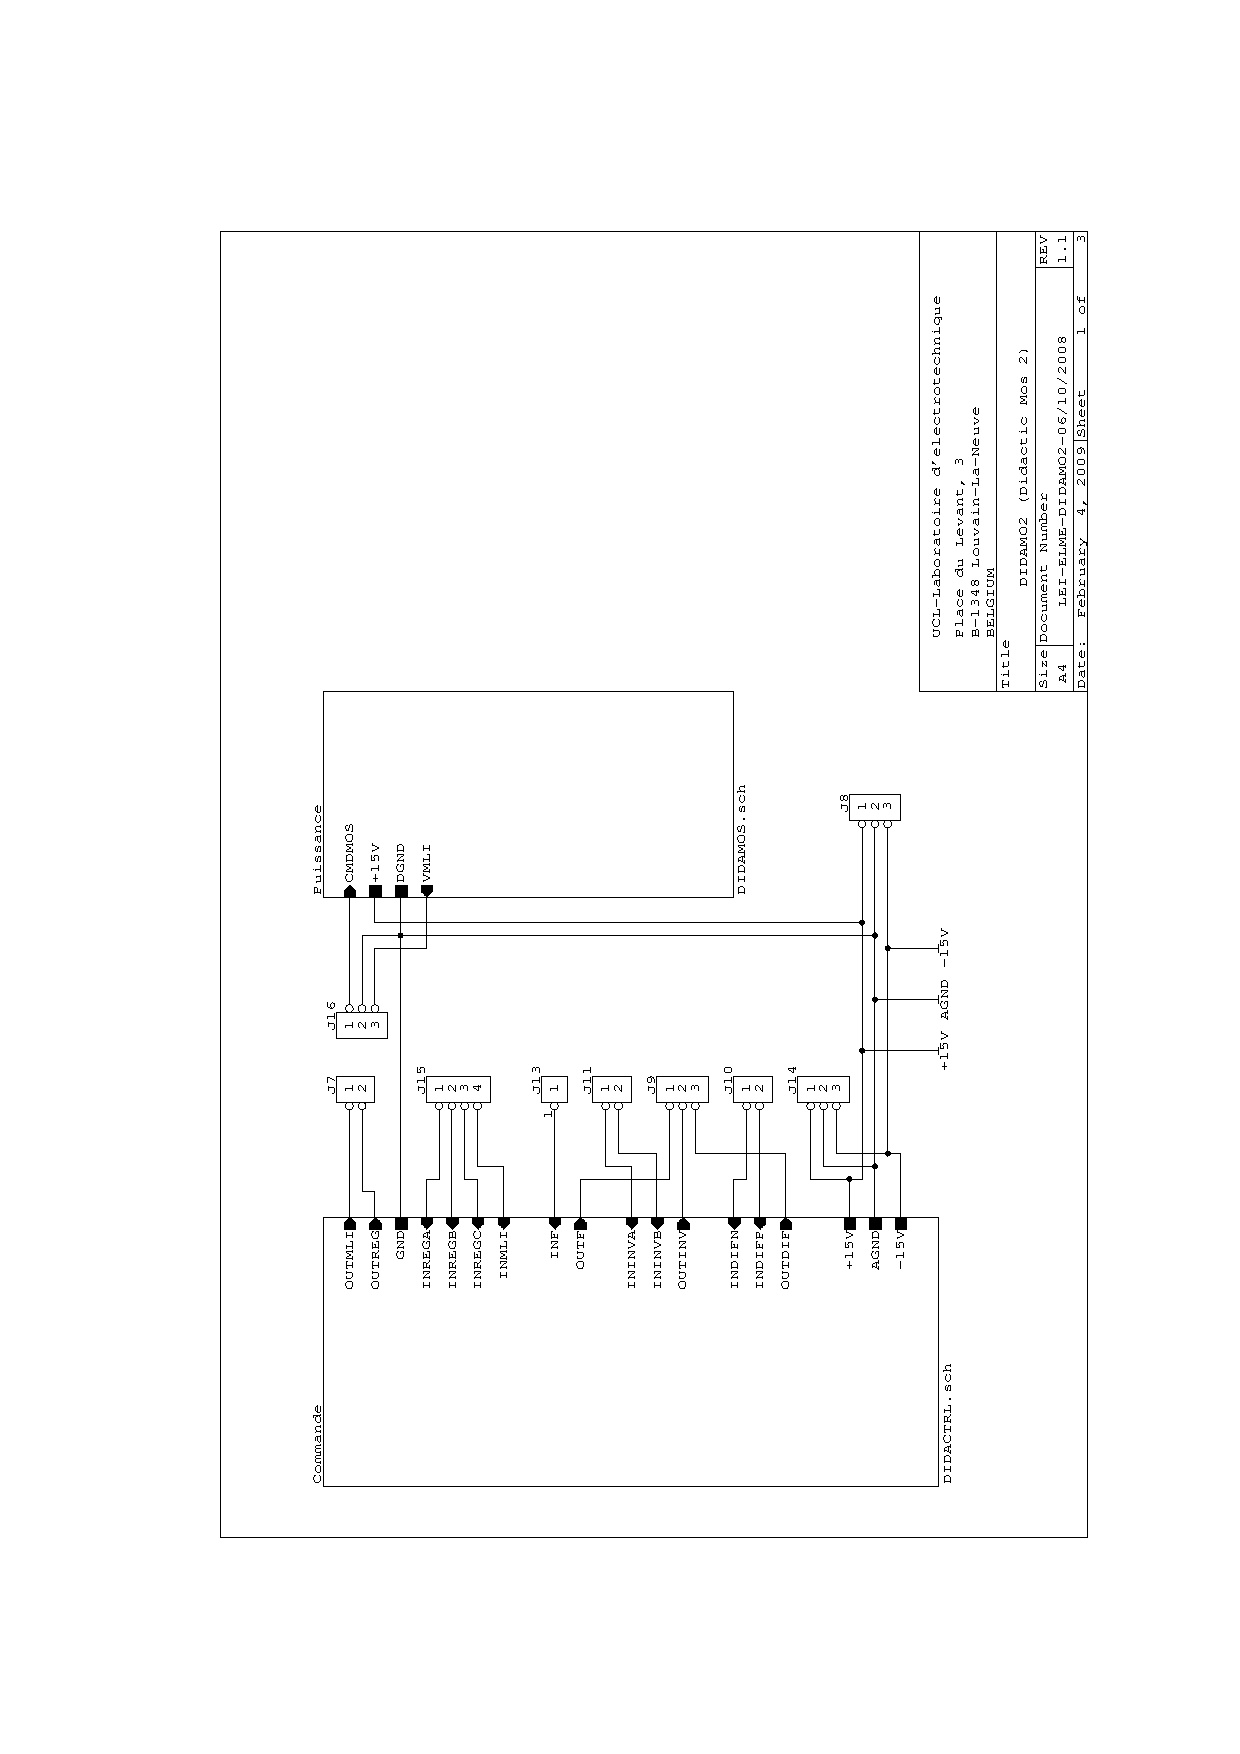
\includepdf[pagecommand=\section{Schéma du circuit DIDAMO2}]{pdf/DIDAMO2.pdf}
\section{Photographie}
\begin{figure}[!ht]
	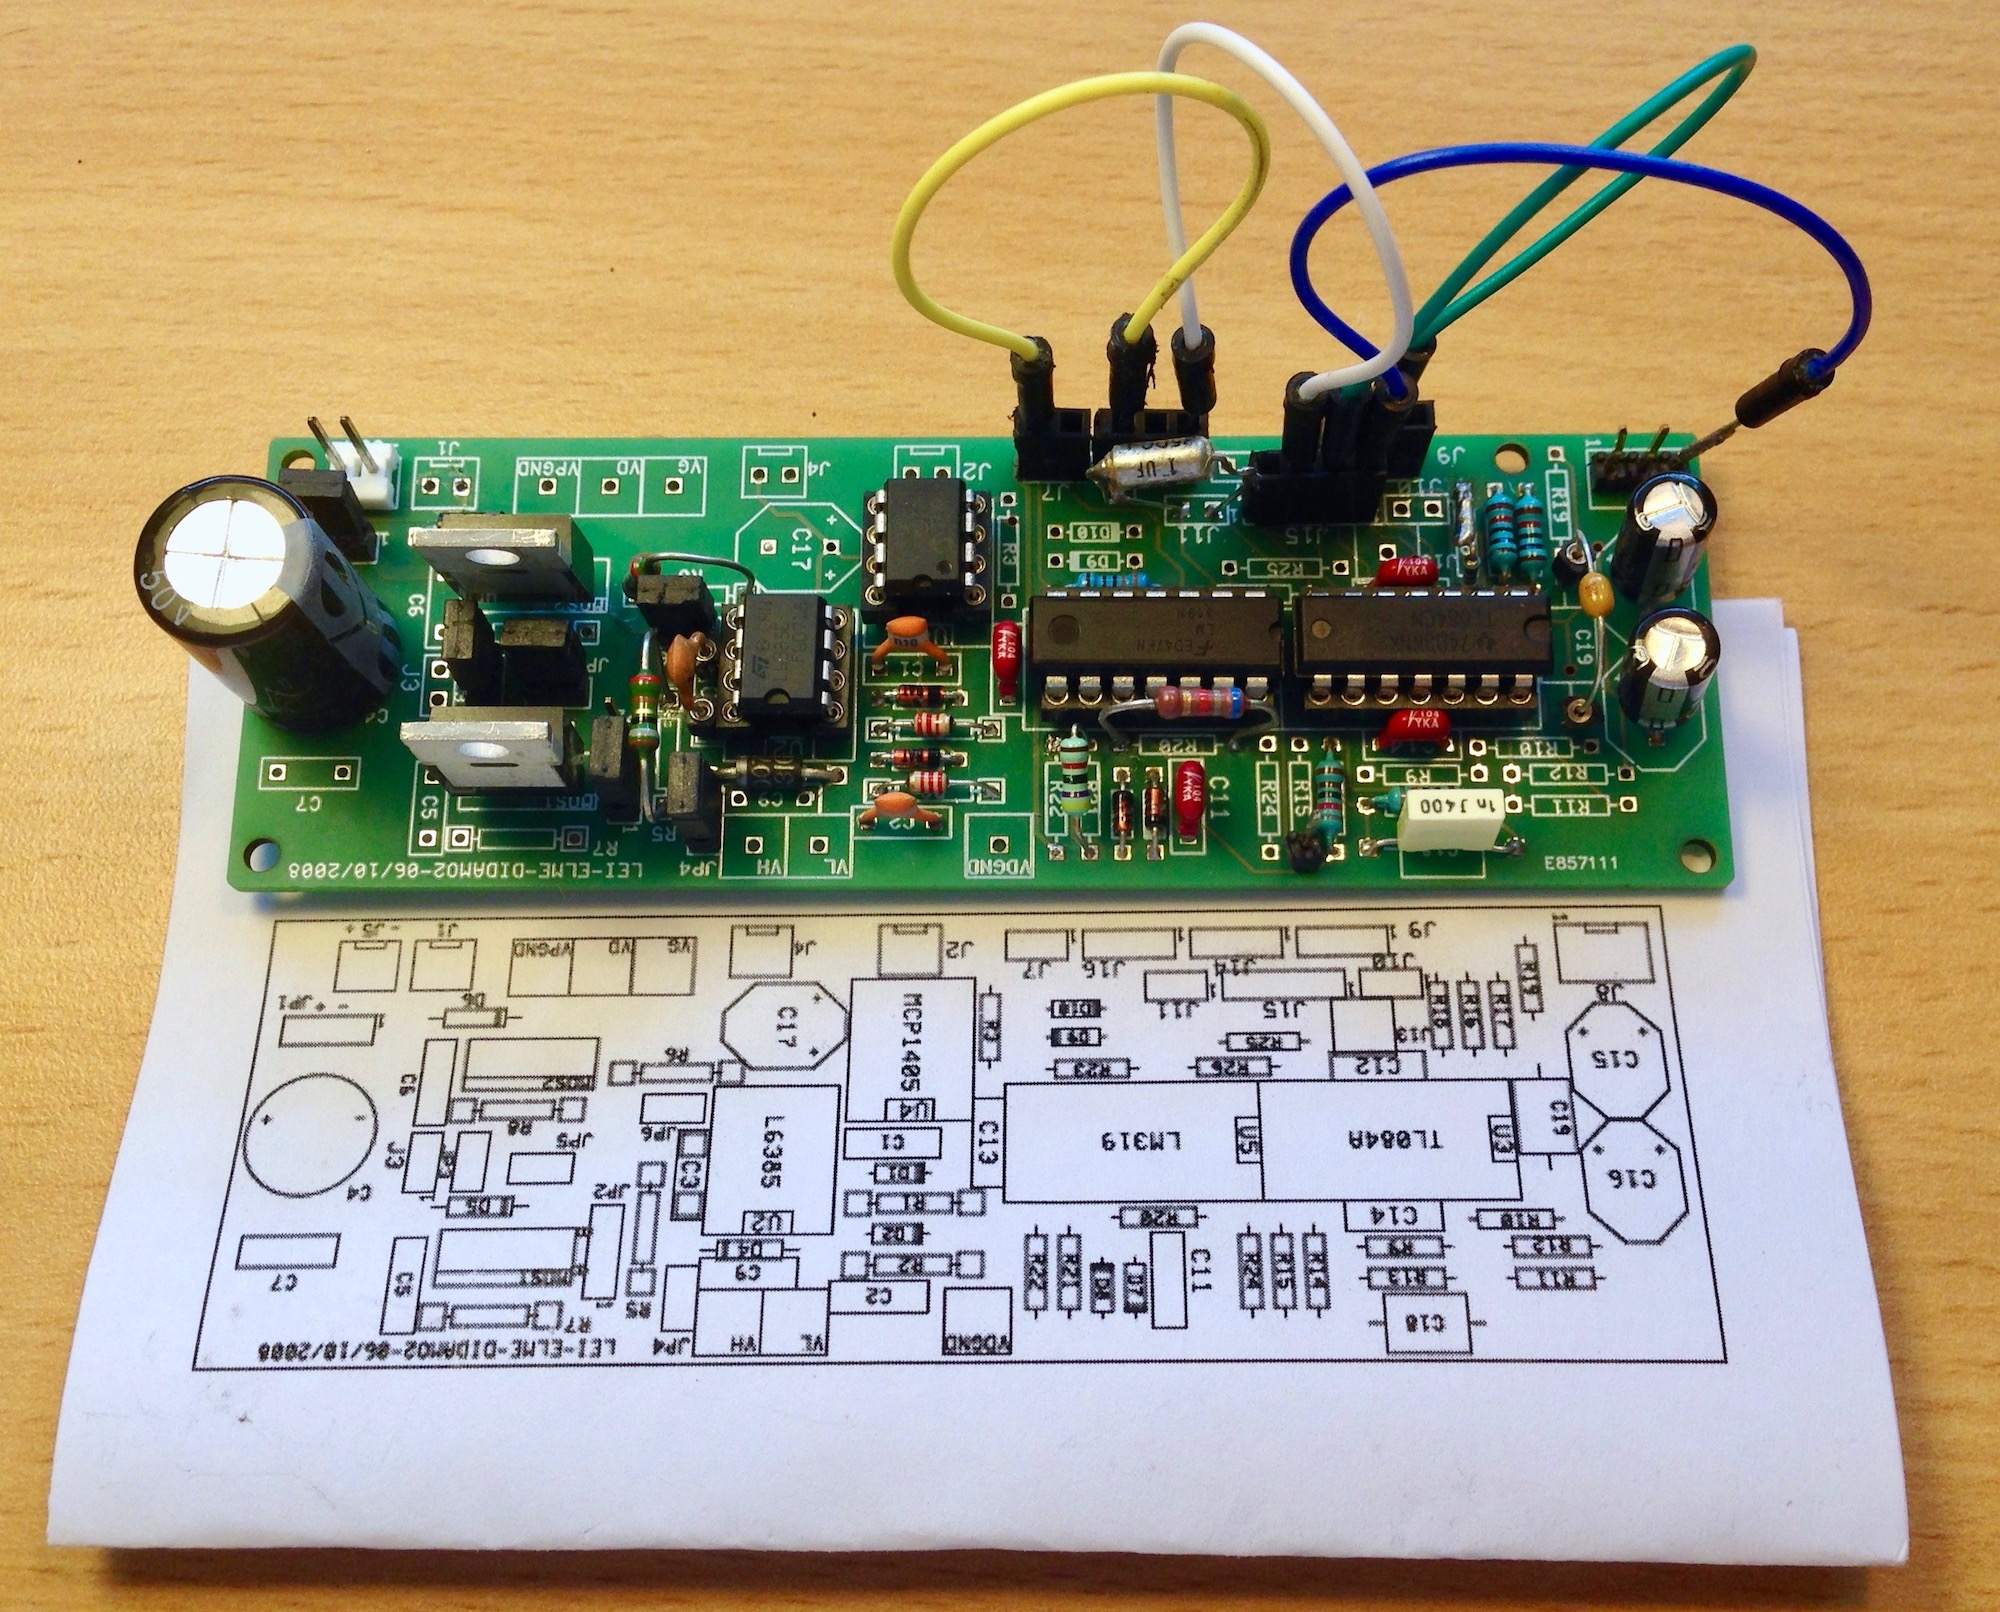
\includegraphics[width=\linewidth]{image/carte.jpg}
	\caption{Photographie prise par le dessus de la carte réalisée.}
\end{figure}

\end{document}
